\documentclass[a4paper,10pt,oneside]{book}

\usepackage[utf8]{inputenc}
\usepackage{float}
%Uma das dificuldades para os usuários do Latex é o posicionamento das figuras, já que ele tenta fazer isso de forma otimizada e automática. Se o usuário quizer forçar as figuras existem duas possibilidades:(1) Definir o posicionamento em: (h) aqui, (t) topo, (b) base, ou na (p) página. O uso do ! siginifica para forçar a solicitação do usuário. a ordem [htb] indica a preferencia que o latex vai re-arranjar as figuras.%(2%) Muitas vezes o usuário não quer otimizar o espaço do texto. Ou seja que posicionar a figura em determinado lugar mesmo que um pedaço da págian fique em branco. Neste caso o indicado é usar o pacote: float e o posicionamento H.%
\usepackage{hyperref}
\usepackage{graphicx}
\usepackage{textcomp}
\usepackage{gensymb}
\usepackage[table,xcdraw]{xcolor}
\usepackage{listings}
\usepackage{cmap}
\usepackage[T1]{fontenc}
\usepackage{verbatim}
\usepackage[table,xcdraw]{xcolor}
\usepackage{longtable}
\usepackage{multirow}

\usepackage[brazil]{minitoc}
\mtcsettitle{minitoc}{Lista de Exemplos}
\newcommand{\filterminitoc}[1]{#1}
\renewcommand{\thesection}{\csname filterminitoc \endcsname{\arabic{chapter}.}\arabic{section}}
\newcommand{\minitocsection}{\begingroup\renewcommand{\filterminitoc}[1]{}\minitoc\endgroup}

% Configurando layout para mostrar codigos C++
\usepackage{listings}
% Definindo novas cores
\usepackage{color}

\usepackage{geometry}
	\geometry{
	a4paper,
	total={170mm,257mm},
	left=40mm,
	right=30mm,
	top=40mm,
	bottom=30mm,
 }

\definecolor{mygreen}{rgb}{0,0.6,0}
\definecolor{mygray}{rgb}{0.5,0.5,0.5}
\definecolor{black}{rgb}{0.3,0.3,0.3}
\definecolor{gray}{rgb}{0.9,0.9,1}
\definecolor{mymauve}{rgb}{0.58,0,0.82}
\lstset{ %
  backgroundcolor=\color{white},  
  basicstyle=\ttfamily\small,            
  breakatwhitespace=false,         
  breaklines=true,                 
  captionpos=b,                    
  commentstyle=\color{mygreen},  
  deletekeywords={...},            
  escapeinside={\%*}{*)},  
  extendedchars=true,    
  %frame=single,	                  
  keepspaces=true,                 
  keywordstyle=\color{blue},       
  language=Octave,,                 
  otherkeywords={*,...},          
  numbers=left,                   
  numbersep=5pt,                   
  numberstyle=\ttfamily\small\color{mygray},
  rulecolor=\color{black},         
  showspaces=false,                
  showstringspaces=false,          
  showtabs=false,                  
  stepnumber=2,                    
  stringstyle=\color{mymauve},  
  tabsize=2,	                   
  title=\lstname,
}


\lstdefinestyle{citacao}{ %
  backgroundcolor=\color{white},   % choose the background color; you must add \usepackage{color} or \usepackage{xcolor}
  basicstyle=\ttfamily,        % the size of the fonts that are used for the code
  breakatwhitespace=false,         % sets if automatic breaks should only happen at whitespace
  breakautoindent=true,
  %breaklines=true,                 % sets automatic line breaking
  columns=fixed,			% don't add spaces between characters
  commentstyle=\color{mygreen},    % comment style
  deletekeywords={...},            % if you want to delete keywords from the given language
  escapeinside={\%*}{*)},          % if you want to add LaTeX within your code
  extendedchars=true,              % lets you use non-ASCII characters; for 8-bits encodings only, does not work with UTF-8
  frame=simple,	                   % adds a frame around the code
  keepspaces=true,                 % keeps spaces in text, useful for keeping indentation of code (possibly needs columns=flexible)
  keywordstyle= \color{blue}\bf,       % keyword style
  language=C,                 % the language of the code
  otherkeywords={*,...},           % if you want to add more keywords to the set
  numbers=left,                    % where to put the line-numbers; possible values are (none, left, right)
  numbersep=5pt,                   % how far the line-numbers are from the code
  numberstyle=\normalfont\color{mygray}, % the style that is used for the line-numbers
  rulecolor=\color{black},         % if not set, the frame-color may be changed on line-breaks within not-black text (e.g. comments (green here))
  showspaces=false,                % show spaces everywhere adding particular underscores; it overrides 'showstringspaces'
  showstringspaces=false,          % underline spaces within strings only
  showtabs=false,                  % show tabs within strings adding particular underscores
  stepnumber=1,                    % the step between two line-numbers. If it's 1, each line will be numbered
  stringstyle=\color{mymauve},     % string literal style
  tabsize=4,	                   % sets default tabsize to 2 spaces
  title=\lstname                   % show the filename of files included with \lstinputlisting; also try caption instead of title
}

\lstdefinestyle{funcao}{ %
  backgroundcolor=\color{white},   % choose the background color; you must add \usepackage{color} or \usepackage{xcolor}
  basicstyle=\ttfamily,        % the size of the fonts that are used for the code
  breakatwhitespace=false,         % sets if automatic breaks should only happen at whitespace
  breakautoindent=true,
  %breaklines=true,                 % sets automatic line breaking
  columns=fixed,			% don't add spaces between characters
  commentstyle=\color{mygreen},    % comment style
  deletekeywords={...},            % if you want to delete keywords from the given language
  escapeinside={\%*}{*)},          % if you want to add LaTeX within your code
  extendedchars=true,              % lets you use non-ASCII characters; for 8-bits encodings only, does not work with UTF-8
  frame=trBL,	                   % adds a frame around the code
  frameround=T,
  rulesep=1pt,
  framesep=5pt,
  rulesepcolor=\color{gray},
  framexleftmargin=-20pt,
  xleftmargin=-20pt,
  xrightmargin=0pt,
  keepspaces=true,                 % keeps spaces in text, useful for keeping indentation of code (possibly needs columns=flexible)
  keywordstyle=\normalcolor\normalfont\normalsize,       % keyword style
  language=C,                 % the language of the code
  otherkeywords={},           % if you want to add more keywords to the set
  numbers=none,                    % where to put the line-numbers; possible values are (none, left, right)
  rulecolor=\color{black},         % if not set, the frame-color may be changed on line-breaks within not-black text (e.g. comments (green here))
  showspaces=false,                % show spaces everywhere adding particular underscores; it overrides 'showstringspaces'
  showstringspaces=false,          % underline spaces within strings only
  showtabs=false,                  % show tabs within strings adding particular underscores
  stringstyle=\color{mymauve},     % string literal style
  tabsize=4,	                   % sets default tabsize to 2 spaces
  title=\lstname                   % show the filename of files included with \lstinputlisting; also try caption instead of title
}




\title{Desenvolvimento em microcontroladores baseados em processadores ARM Cortex-M4 com TivaWare}
\author{
        Leandro Fabian Junior\\
        \and
        Callebe Soares Barbosa\\
        \and
        Orientador: Gustavo Weber Denardin
}
\date{2016}


%renomeia o titulo dos tipos figure
\renewcommand{\figurename}{Figura}
%renomeia o titulo dos tipos Table
\renewcommand{\tablename}{Tabela} 
\renewcommand{\lstlistingname}{Código} 
\renewcommand{\chaptername}{Capítulo}
\renewcommand{\contentsname}{Índice}
\renewcommand{\bibname}{Referências}
\renewcommand{\listfigurename}{Lista de Figuras}
\renewcommand{\listtablename}{Lista de Tabelas}

\graphicspath{{figuras/}{fig_site/}}

\newcommand{\ttbu}[1]{\texttt{\textbf{\underline{#1}}}}

\usepackage{ifthen}

\newcommand{\forloop}[5][1]%
{%
\setcounter{#2}{#3}%
\ifthenelse{#4}%
	{%
	#5%
	\addtocounter{#2}{#1}%
	\forloop[#1]{#2}{\value{#2}}{#4}{#5}%
	}%
% Else
	{%
	}%
}%

% How to use:    \forloop[step]{counter}{initial_value}{conditional}{code_block}
% 
% For example:
% 
% \newcounter{ct}
% \forloop{ct}{1}{\value{ct} < 5}%
% {%
% \arabic{ct}
% }



\begin{document}
%\maketitle

\begin{titlepage}
	\newgeometry{left=3cm, bottom=3cm, right=3cm, top=3cm}
	\centering
% 	\begin{minipage}{1\textwidth}
% 	\begin{multicols}{2}	
% 	\begin{minipage}{.5\textwidth}
% 		\begin{flushright}
% 			\begin{center}
% 			
\includegraphics[width=.9\textwidth]{logo_utfpr.png}\par\vspace{1cm}
% 			\end{center}
% 		\end{flushright}
% 	\end{minipage}
% 	\begin{minipage}{.5\textwidth}
% 		\begin{flushleft}
% 			\scshape \LARGE Universidade Tecnológica Federal do Paraná\par
% 		\end{flushleft}
% 	\end{minipage}
% 	\end{multicols}
% 	\end{minipage}

\includegraphics[width=.3\textwidth]{logo_utfpr.png}\par\vspace{10pt}
\rule{\textwidth}{1pt}
{\scshape \LARGE Universidade Tecnológica Federal do Paraná\par\vspace{5pt} \Large Campus Pato Branco}
	\rule{\textwidth}{1pt}
	\vfill
	{\huge\bfseries Desenvolvimento em microcontroladores baseados em processadores ARM Cortex-M4\par}
	\vfill
	\begin{minipage}{\textwidth}
		\centering
		\Large\itshape Leandro Fabian Junior\par
		\Large\itshape Callebe Soares Barbosa\par
	\end{minipage}
	\vspace{2cm}
	
	{orientado por\par
	\Large\itshape Gustavo Weber Denardin}

	\vfill

% Bottom of the page
	{\large2016\par}
	\newpage
	\pagenumbering{gobble}
 \vfill
  \begin{center}
   {\scshape \LARGE Universidade Tecnológica Federal do Paraná\par\vspace{5pt} \Large Campus Pato Branco} \\[2.5cm]

   \begin{minipage}{\textwidth}
		\centering
		\Large\itshape Leandro Fabian Junior\par
		\Large\itshape Callebe Soares Barbosa\par
	\end{minipage}
	\vspace{1cm}
	
	{orientado por\par
	\Large\itshape Gustavo Weber Denardin}
	\vfill

   {\huge\bfseries Desenvolvimento em microcontroladores baseados em processadores ARM Cortex-M4\par}
   \vfill

   \hspace{.45\textwidth} %posiciona a minipage
   \begin{minipage}{.5\textwidth}
   \large Recurso Educacional Aberto produzido com o fomento do Programa de Bolsas para o Desenvolvimento de Recursos Educacionais Abertos (PIBEA) por meio do Programa de Bolsas de Fomento às Ações de Graduação da UTFPR.
  \end{minipage}
  \vfill
  \hspace{11cm}
  
\includegraphics[width=3cm]{Cc-by-nc-sa_icon.png}
	
\vspace{2cm}

{\large2016\par}
\end{center}
\end{titlepage} 

\pagenumbering{arabic}
\setcounter{page}{2}
\listoffigures
\listoftables

\dominitoc
\nomtcrule
\tableofcontents

\chapter{Introdução}
Este texto busca iniciar o leitor no desenvolvimento em plataformas baseadas em processadores com arquitetura ARM.

O Hardware utilizado para os exemplos aqui apresentados será o Kit de 
avaliação da Texas Instruments Tiva\textsuperscript{TM} C Series TM4C1294.

\chapter{Conhecendo o Processador ARM}
\section{Características ARM}

O termo ARM se refere a \emph{Advanced RISC Machine}, ou seja uma arquitetura que usa o conceito conhecido como RISC. RISC, \emph{Reduced Instruction Set Computer}, é uma linha de arquitetura que favorece um conjunto simples e pequeno de instruções que levam aproximadamente a mesma quantidade de tempo para serem executadas, permitindo que estes processadores tenham menos transístores do que aqueles projetados na arquitetura convencional. Logo essa abordagem reduz a liberação de calor, o consumo de energia e a quantidade de componentes em um processador.

A arquitetura dos processadores usados aqui, o Cortex-M3 e Cortex-M4, são ambos as implementações da arquitetura ARMv7-M. Existem diferentes tipos de arquitetura ARM para diferentes tipos de processadores, que ainda podem variar conforme são atualizadas ao longo dos anos. Os detalhes da arquitetura ARMv7-M estão documentados no Manual de Referência da Arquitetura  ARMv7-M, disponível no site da  \href{http://infocenter.arm.com/help/index.jsp}{ARM Limited}.

O Cortex-M3 e Cortex-M4 são essencialmente idênticos em seus aspectos construtivos, de modo que o diagrama de blocos da figura \ref{DiagramaDeBlocosARM}  apresenta uma visão  geral interna adequada tanto do processador Cortex –M4 quanto -M3.

\begin{figure}[h]
	\centering
	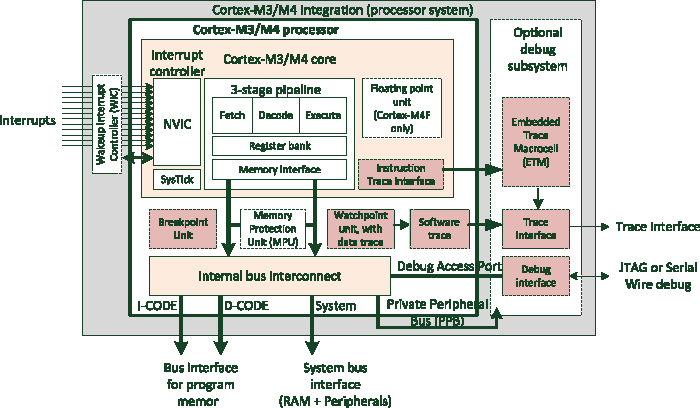
\includegraphics[scale=0.9]{DiagramaDeBlocosARM}
	\caption{Diagrama de Blocos - Processador Cortex-M3 e Cortex-M4 \cite{DATASHEET_TIVA}}
	\label{DiagramaDeBlocosARM}
\end{figure}

Na figura \ref{DiagramaDeBlocosARM} notamos a presença de elementos no processador como:  o controlador de vetores de interrupção, NVIC (\emph{Nested Vectored Interrupt Controller}); o controlador de acionamento de interrupção, WIC (\emph{Wakeup Interrupt Controller}); o temporizador SysTick; a unidade de proteção de memória MPU (\emph{Memory Protection Unit}); e uma unidade de ponto flutuante presente apenas no Cortex –M4. Existe ainda um sistema de debug dentro do processador para realizar depuração de software e um sistema interno de barramentos para transferência de dados entre o núcleo do processador, o sistema de debug e o MPU. 

Os processadores da família Cortex M são de 32 bits, podendo também trabalhar com dados de 8 bits e 16 bits de forma bastante eficiente. Já os processadores Cortex-M3  e Cortex-M4, mesmo sendo da família Cortex M, podem realizar uma série de operações envolvendo dados de 64 bits. Estas operações podem ser realizadas através de um \emph{piperline} de três estágios com uma arquitetura de barramento do tipo \emph{Harvard} permitindo instruções simultâneas de busca e acesso de dados.

Uma das grandes vantagens dos processadores Cortex M é seu baixo consumo de energia. Em especial os processadores Cortex M3 e Cotex M4 podem executar instruções com taxa de $200 mA/MHz$ com alimentação de $1,8 V$. Estes processadores possuem modos de suspensão que tornam possíveis desativar dispositivos de \emph{Clock} para economizar energia, e um \emph{hardware} adicional para despertar o processador dos modos de suspensão.

Devemos salientar aqui que estamos sempre nos referindo a apenas aos processadores, e que este é uma parte constituinte do microcontrolador. De modo que os demais componentes da placa são desenvolvidos pelos diferentes fabricantes. Assim existem vários tipos de microcontroladores com diferentes características de periféricos e recursos, porém a arquitetura empregada nos processadores é a mesma.


\section{Modos de operação ARM Cortex-M4}

O processador Cortex-M4 possui dois estados de operação, como mostrado na figura \ref{fig:modosDeOperacao}, \emph{debug state} e \emph{Thumb state}. O \emph{debug state} ocorre quando o processador é interrompido, por exemplo ao atingir um \emph{breakpoint}, então a execução de instrução é interrompida. Já o \emph{Thumb state} ocorre quando o código do programa está sendo executado. Diferente de outros processadores ARM, o Cortex-M não suporta instruções ARM.

\begin{figure}[H]
	\centering
	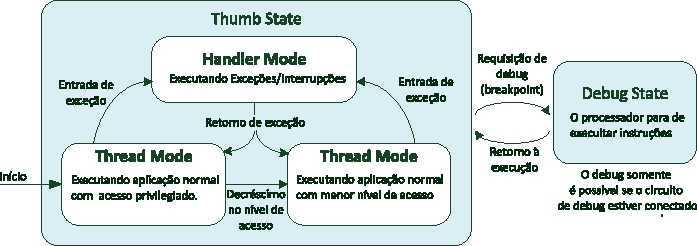
\includegraphics[scale=0.9]{modosDeOperacaoCortex-M4}
	\caption{Modos de Operação \cite{DATASHEET_TIVA}}
	\label{fig:modosDeOperacao}
\end{figure}

No \emph{Thumb state} ainda existem dois modos de operação, que dizem respeito ao nível de privilégio no acesso ao processador. Ao executar uma rotina de tratamento de interrupção o processador entra em um nível de acesso privilegiado, caracterizando o \emph{handler mode}. Durante a execução de uma aplicação normal o processador pode estar tanto em nível de acesso privilegiado quanto em nível menor, sendo chamado de \emph{thread mode}. Isso é controlado por um registrador específico. 

A aplicação pode alterar seu nível de acesso durante o \emph{thread mode}, para um nível menos privilegiado. Porém, para aumentar seu nível de acesso deve haver um mecanismo de exceção/interrupção por parte do processador.  Tais mecanismos de controle de nível de acesso garantem uma maior robustez para o sistema, controlando o acesso à regiões críticas de memória.

\section{Registradores internos}

Para um controle melhor e um processamento de dados maior o Cortex-M4 possui registradores internos ao processador agrupados em um conjunto chamado de \emph{banco de registradores}. Cada instrução enviada ao processador especifica a operação a ser executada, os registradores fonte e se necessário os registradores de destino. A arquitetura ARM é baseada no modelo conhecido como \emph{load/store}, ou seja, para processar um conteúdo que esteja na memória é preciso carregá-lo para um registrador interno e então processá-lo. Se necessário, é preciso armazená-lo de volta na memória.

\begin{figure}[H]
	\centering
	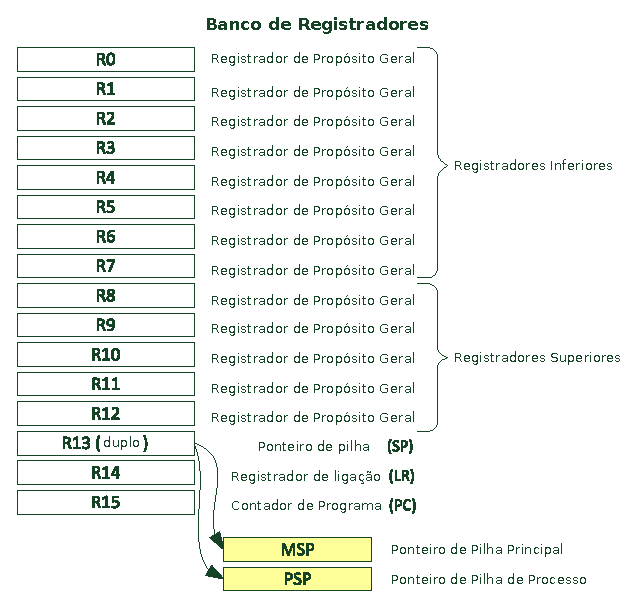
\includegraphics[scale=0.9]{bancoRegistradores}
	\caption{Banco de registradores internos \cite{DATASHEET_TIVA}}
	\label{fig:bancoRegistradores}
\end{figure}

O banco de registradores do Cortex-M4 possui 16 registradores de 32 bits, como mostrado na Figura \ref{fig:bancoRegistradores}. Cada registrador possui seu propósito, como detalhado a seguir:

\begin{description}
\item[R0 - R12: Registradores de Propósito Geral]\hfill \\
Devido ao número limitado no conjunto de instruções, muitas das de 16 bits somente acessam os registradores de R0 à R7, chamados de \emph{registradores inferiores}. De R8 à R9, os \emph{registradores altos}, podem ser usados com as instruções de 32 de bits e alguns com instruções 16 de bits. Os valores iniciais desses registradores são indefinidos.

\item[R13: Ponteiro de Pilha (\emph{Stack Pointer}, SP)]\hfill \\
Usado para acessar a pilha de memória. Fisicamente há dois ponteiros de pilha, o principal (\emph{Main Stack Pointer}, MSP) e o de processo (\emph{Process Stack Pointer}, PSP)). O MSP é o ponteiro padrão, é selecionado após um \emph{reset} do sistema ou quando o processador está em modo de exceção (Handler Mode). Seu valor inicial é o primeiro da memória na sequência de \emph{reset}. Já o PSP é usado durante o Thread Mode, quando as tarefas da aplicação estão rodando, seu valor inicial é desconhecido.

Somente um dos ponteiros de pilha é visível durante a aplicação e os dois bits menos significativos de ambos são sempre nulos. Em aplicações que não fazem uso de um sistema operacional somente o MSP é usado.

\item[R14: Registrador de Ligação (\emph{Link Register}, LR)]\hfill \\
Esse registrador armazena automaticamente o ponto em que uma rotina chama uma sub-rotina. Assim, ao fim da execução dessa sub-rotina, esse valor é carregado para o Contador de Programa e a execução continua de onde tinha anteriormente parado.

Se uma sub-rotina chamar outra sub-rotina, o valor nesse registrador será substituído e o ponto de retorno antigo se perderá, portanto é preciso que esse último valor seja salvo na pilha de memória.

Durante uma rotina de tratamento de exceção, o valor de LR é também sobrescrito mas por um valor de retorno de exceção, usado para disparar o retorno da exceção ao fim da rotina de tratamento.

\item[R15: Contador de Programa (\emph{Program Counter, PC})]\hfill \\
Marca o próximo endereço que deve ser executado na aplicação. Quando este registrador é lido, automaticamente seu valor decrementa de 4 (32 bits), apontando para o próximo endereço da execução. Já quando é feito uma operação de escrita, o programa pula para a posição apontada e passa a executar a aplicação a partir deste novo ponto.

O bit menos significativo do PC indica o tipo de instrução que está sendo executada, '0' para ARM e '1' para Thumb. Portanto no Cortex-M4, tal bit deve ser sempre '1' pois não são suportadas instruções ARM. Este fato deve ser lembrado quando é feita uma operação de escrita sobre o registrador.

\end{description}





\chapter{Conhecendo a plataforma de trabalho}
O hardware utilizado aqui será o  TIVA \texttrademark ~~ TM4C1294NCPDT, um kit de desenvolvimento da empresa Texas Instruments que possui um microcontrolador baseado no processador ARM Cortex-M4. A tabela \ref{tab:CaracteristicasMicro} traz suas principais características.

%% TABELA DE CARACTERISTICAS BASICAS %%%%%%%%%%

% \begin{table}[!h]
% \centering

\begin{longtable}{|l|l|}

\hline
\cellcolor[HTML]{343434} \color[HTML]{FFFFFF} Características & \cellcolor[HTML]{343434} \color[HTML]{FFFFFF} Descrição \\
\hline
Núcleo & ARM Cortex-M4F\\
\hline
Performance & Operação até 120-MHz; 150 DMIPS \\
& (Dhrystone MIPS) de performance \\
\hline
Memória Flash & 1024 KB  \\
\hline
SRAM & 256 KB single-cycle System SRAM \\
\hline
EEPROM & 6KB  \\
\hline
ROM & ROM interna carregada com biblioteca  \\
 & TivaWare™  C Series \\
\hline
Interface de Periféricos Externos (EPI)  & Interface dedicada de 8-/16-/32-   \\ 
 &  bits dedicados a periféricos e memoria\\
\hline
 Verificação de Redundância & Função Hash de 16-/32- bits,  que suporta  \\
  Cíclica (CRC)   & quatro formas de CRC \\
\hline
\begin{comment}
 Função de Adulteração & Suporte para quatro entradas de  \\
 & adulteração e resposta de evento de  \\
 & adulteração configurável configurável  \\
\hline
\end{comment}
Universal Asynchronous  & 8 módulos UARTs \\
Receivers/Transmitter (UART) & \\
\hline
Quad Synchronous Serial & Quatro módulos de SSI com Bi- , Quad-\\
Interface (QSSI) &  e suporte avançado de SSI\\
\hline
Inter-Integrated Circuit ($I^{2}C$) & 10 módulos $I^{2}C$ com 4 velocidades \\
 & de transmissão\\
\hline
Controller Area Network (CAN) & 2 controladores CAN 2.0 A/B \\
\hline
Ethernet MAC & 10/100 Ethernet MAC \\
\hline
Ethernet PHY & PHY com IEEE 1588 PTP \\
\hline
Universal Serial Bus (USB) & USB 2.0 OTG/Host/Device  \\ 
& com ULPI interface e suporte a Link   \\
& Power Management (LPM) \\
\hline
Micro Acesso Direto à Memória ($\mu DMA$) & Controlador ARM$\copyright$ PrimeCell$\copyright$  \\
& 32-channel configurável  $\mu DMA$ \\
\hline
General-Purpose Timer (GPTM) & 8 blocos 16/32-bit GPTM \\
\hline
Watchdog Timer (WDT) & 2 Watchdog Timers \\
\hline
Hibernation Module (HIB) & Low-power battery-backed \\
 & Hibernation module \\
\hline
General-Purpose Input/Output (GPIO) & 15 physical GPIO blocks \\
\hline
Pulse Width Modulator (PWM) & 1 modulo PWM , com 4 geradores PWM  \\
 & e um  registador de controle,\\
 &  com um total de 8  saídas PWM.\\
\hline
Quadrature Encoder Interface (QEI) & Um modulo QEI \\
\hline
Analog-to-Digital Converter (ADC) & 2 modulos ADC de 12-bit\\
 & taxa de 2 milhões de amostras/segundo\\
\hline
Controlador Comparador Analógico & Três comparadores analógicos \\
& independentes \\
\hline
Comparador Digital & 16 comparadores digitais \\
\hline
JTAG e Serial Wire Debug (SWD) & 1 modulo JTAG  com ARM SWD\\
& integrado \\
\hline
Encapsulamento & 128-pin TQFP \\
\hline
Temperatura de Operação & $-40 \degree C$ até $105 \degree C$ \\
\hline
\caption{Características Básicas - TM4C1294NCPDT \cite{DATASHEET_TIVA}}
\label{tab:CaracteristicasMicro}
\end{longtable}
% \end{table}

%%%%%%%%%%%%%%%%%%%%%%%%%%%%%%%%%%%%%%%%%%%%%%%%%%%%%%%


O TM4C1294NCPDT possui dois barramentos. Um desses é responsável pela conexão padrão entre o núcleo de processamento e os periféricos, o \emph{Advanced Peripheral Bus} (APB). Já o outro, o \emph{Advanced High-Performance Bus} (AHB), é um barramento especial que pode ser requisitado da maioria dos periféricos e, possui uma resposta muito mais rápida por ser exclusivo. O esquema dos barramentos é mostrado no diagrama de blocos da figura \ref{fig:DiagramaBlocosTiva}.


\begin{figure}[H]
\centering
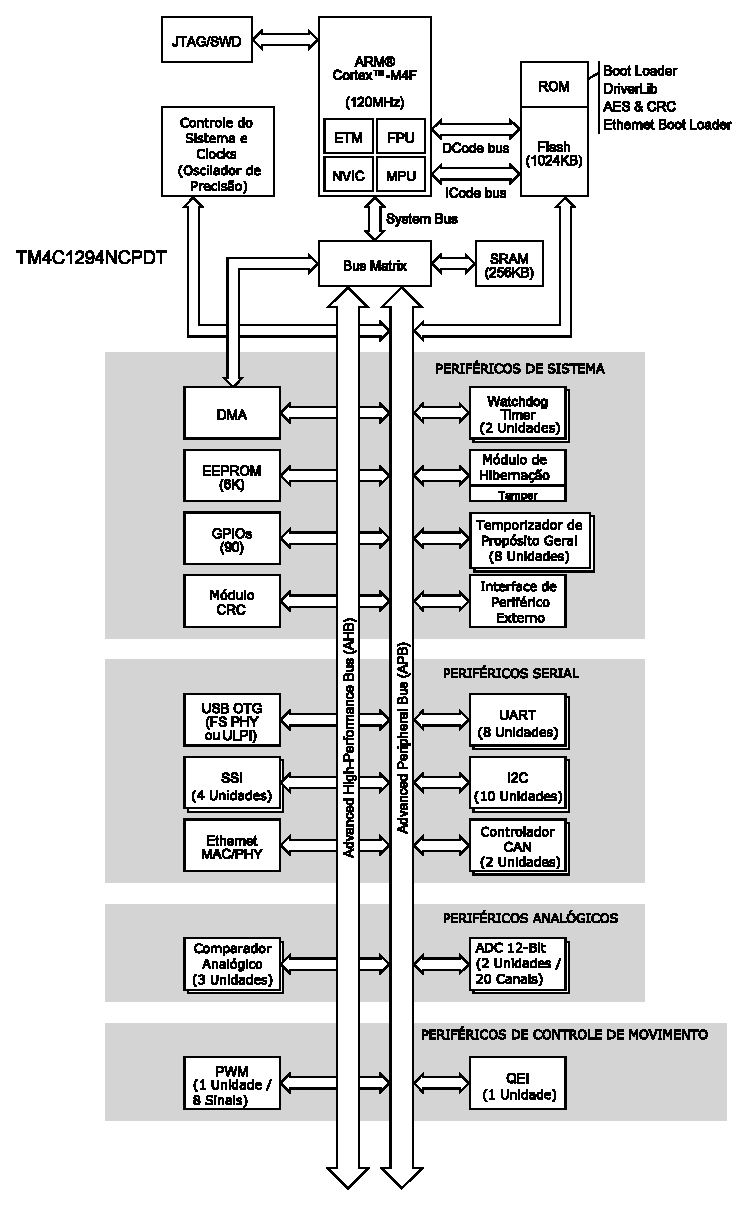
\includegraphics[width=0.8\textwidth] {DiagramaBlocosTiva.eps}
    \caption{Diagrama de Blocos - TM4C1294NCPDT \cite{DATASHEET_TIVA}}
    \label{fig:DiagramaBlocosTiva}
\end{figure}

%%%%%%%%%%%%%%%%%%%%%%%%%%%%%%%%%%%%%%%%%%%%%%%%%%%%%%%

\chapter{Iniciando um projeto no Code Composer}
Os projetos abordados adiante farão uso da IDE Code Composer que é baseada em Eclipse em sua versão 6.1.2 que é a mais recente no momento em que este texto é escrito. oferecida gratuitamente mediante a um cadastro realizado no site da Texas Instruments.

Na hora de instalar a IDE é preciso que sejam marcadas as opções de compatibilidade com a placa em uso, a Tiva C Series TM4C1294 Connected LaunchPad, e ainda seu compilador GCC, caso contrário o projeto não poderá ser criado.

Após iniciar o Code Composer, inicie um novo projeto em \textbf{File $>$ New $>$ CCS Project} como mostrado na Figura \ref{fig:novoProjeto01}.

\begin{figure}[H]
	\centering
	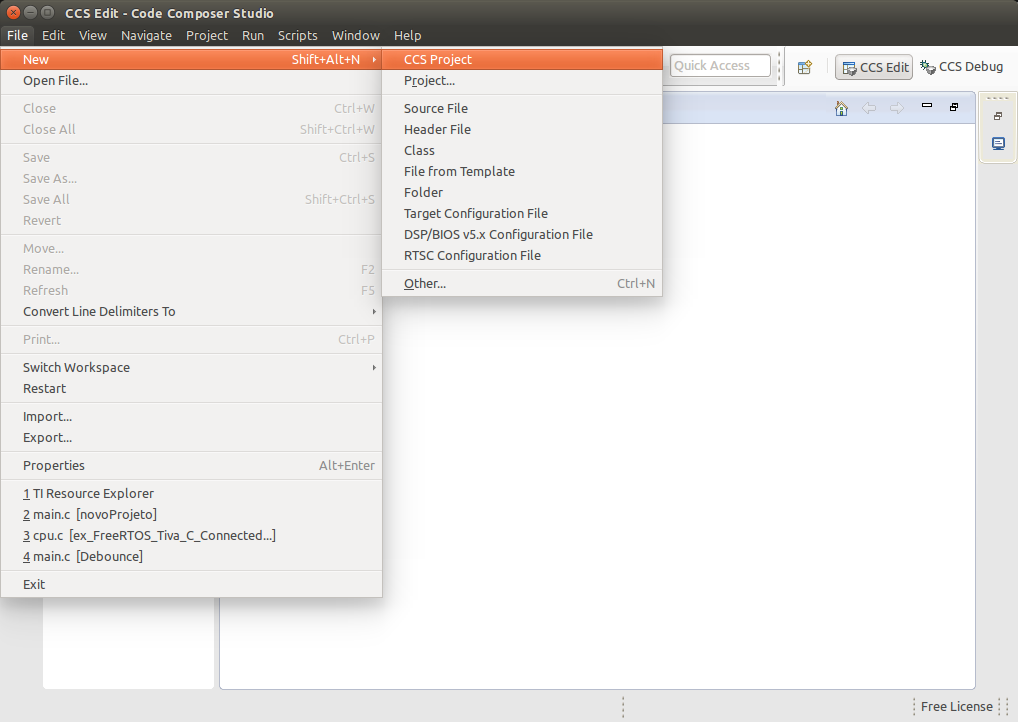
\includegraphics[scale=0.35]{novoProjeto01.png}
	\caption{Criando um novo projeto}
	\label{fig:novoProjeto01}
\end{figure}

Uma janela de configurações será exibida para que o ambiente seja preparado 
para o hardware em uso, como na Figura \ref{fig:novoProjeto02}.

Para o hardware aqui utilizado, em \emph{Target} escolhe-se a opção 
\textbf{Tiva C Series} e no segundo campo \textbf{Tiva TM4C1294NCPDT}.

Em \emph{Connection} será utilizada a \textbf{Stellaris In-Circuit 
Debug Interface} para a programação e debug do microcontrolador.

Após isso, escolhe-se um nome para o projeto e o diretório que será armazenado, 
que é normalmente o local do workspace padrão marcando a opção \textbf{Use 
default location}.

A Texas Instruments disponibiliza um compilador próprio porém será usado aqui o 
GCC, compilador de código aberto sob a licença GNU. Portanto, em \emph{Compile 
version} escolhe-se a opção \textbf{GNU} com a versão mais recente.
As outras opções não precisam ser alteradas.

\begin{figure}[H]
	\centering
	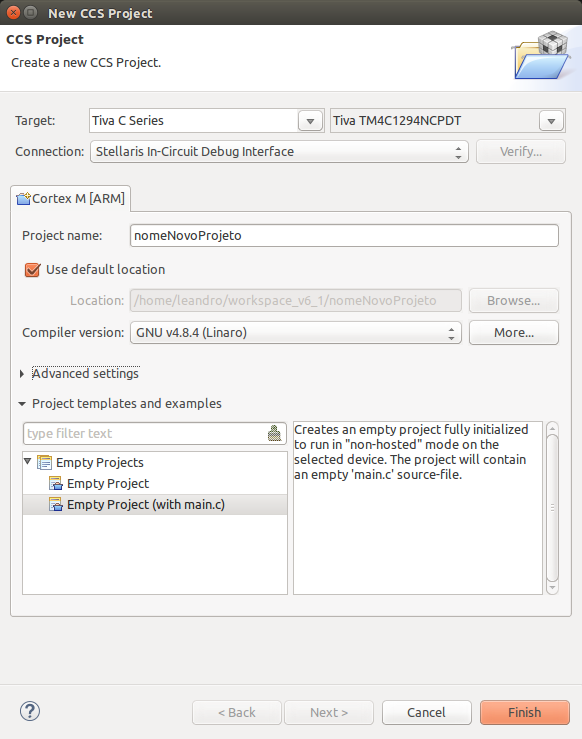
\includegraphics[scale=0.5]{novoProjeto02.png}
	\caption{Configurando o projeto}
	\label{fig:novoProjeto02}
\end{figure}

Clicando em \emph{Finish} o projeto será criado. Para o correto funcionamento 
do compilador GCC devem-se ainda ser feitos mais alguns ajustes.

Selecionando o projeto criado na barra lateral \emph{Project Explorer}, vá em 
\textbf{Project $>$ Properties} como na Figura \ref{fig:novoProjeto03}.

\begin{figure}[H]
	\centering
	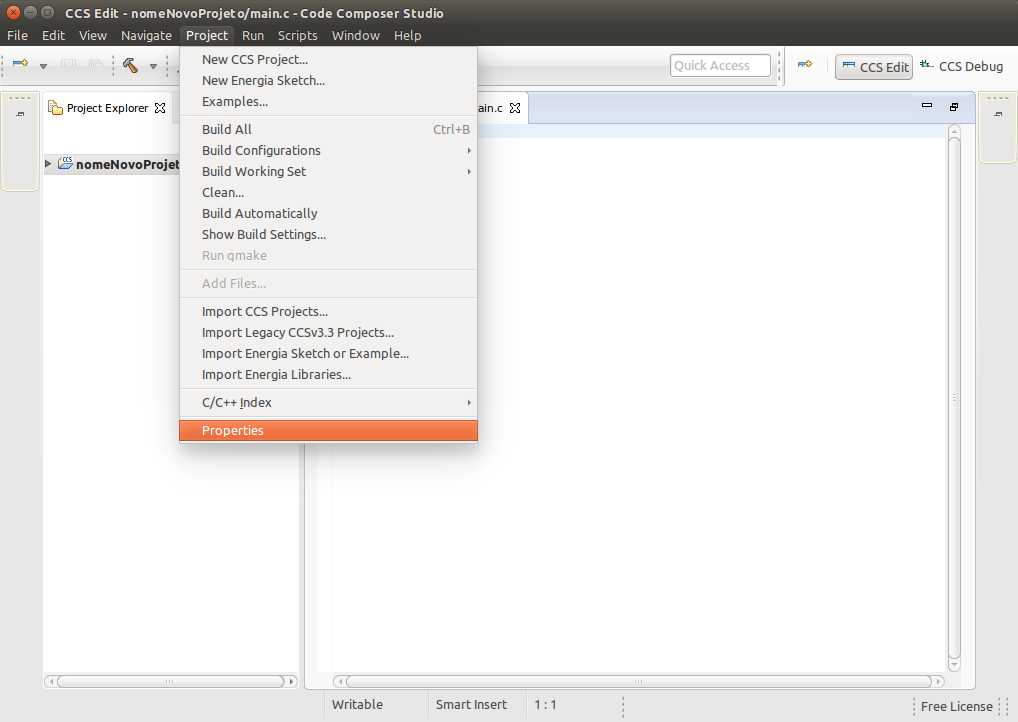
\includegraphics[scale=0.35]{novoProjeto03.png}
	\caption{Abrindo propriedades do projeto}
	\label{fig:novoProjeto03}
\end{figure}

Na janela de propriedades selecione \textbf{Build $>$ GNU Compiler $>$ 
Symbols}. Adicione um novo símbolo clicando no botão \emph{Add} como na Figura 
\ref{fig:novoProjeto04}. Na janela que se abre digite 
\textbf{TARGET\_IS\_TM4C129\_RA1} e clique em \emph{OK}. Adicione ainda o 
símbolo \textbf{gcc}. Esses símbolos não podem conter erros de escrita, caso 
contrário causarão erros na hora da compilação. Ao se ter os três símbolos 
mostrados na Figura \ref{fig:novoProjeto04}, selecione \textbf{Build $>$ GNU 
Linker $>$ Basic}. Na opção \emph{Set start address} digite \textbf{\_start} 
como na Figura \ref{fig:novoProjeto05} e clique em \emph{OK}.

\begin{figure}[H]
	\centering
	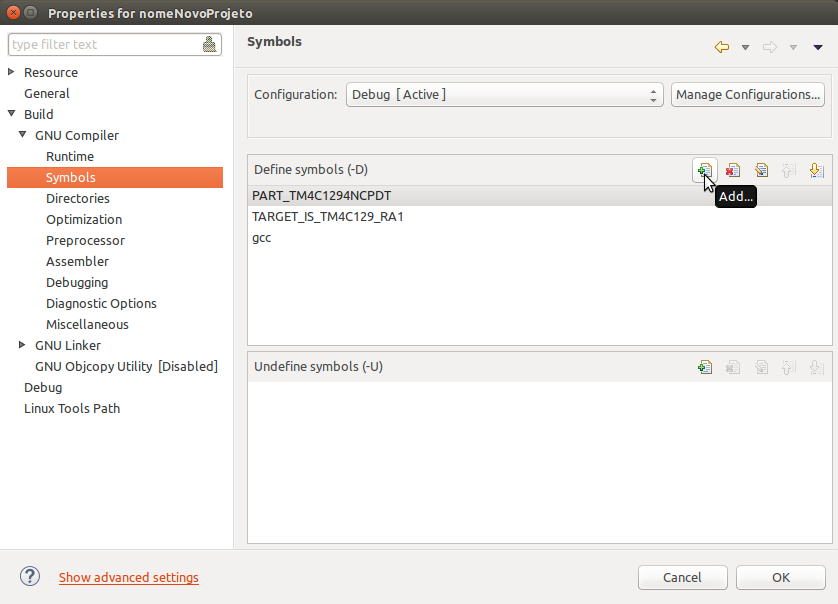
\includegraphics[scale=0.4]{novoProjeto04.png}
	\caption{Adicionando símbolo para a compilação no GCC}
	\label{fig:novoProjeto04}
\end{figure}

\begin{figure}[H]
	\centering
	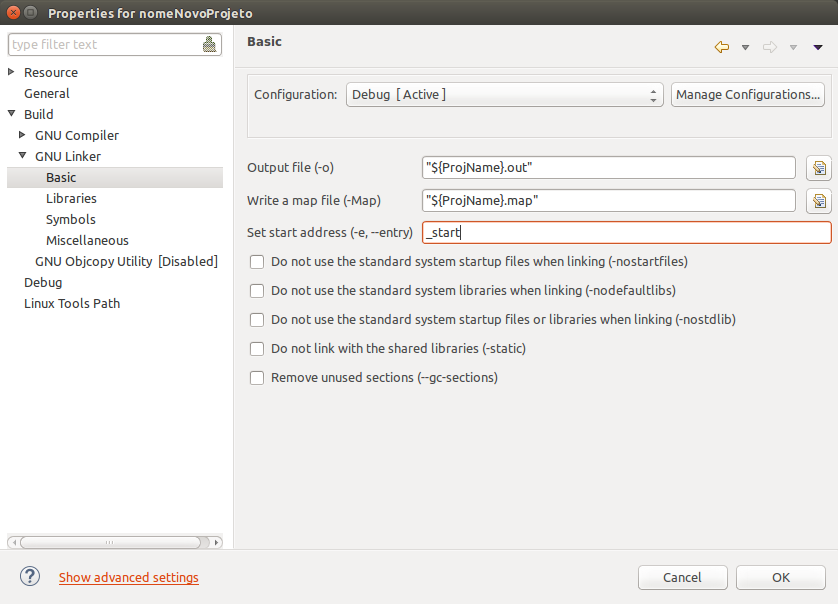
\includegraphics[scale=0.4]{novoProjeto05.png}
	\caption{Configurando endereço de início do Linker do GCC}
	\label{fig:novoProjeto05}
\end{figure}

Ao fim desses passos o projeto estará criado e poderá ser compilado no Code Composer utilizando o GCC.

\chapter{Biblioteca TivaWare}
Para facilitar a programação do microcontrolador será feito o uso da biblioteca TivaWare fornecida pela Texas Instruments. Tal ferramenta facilita o controle do processador e acesso aos periféricos disponíveis. A TivaWare pode ser obtida no site da empresa gratuitamente.

O site disponibiliza somente a versão para o sistema Windows, que vem em formato executável, sendo preciso apenas dar um clique duplo sobre o arquivo e seguir os passos da instalação. Já para sistemas não derivados do \emph{MS-DOS}, basta abrir este mesmo executável baixado com um aplicativo de descompactação de arquivos e copiar o conteúdo para um diretório qualquer desejado.

A estrutura do TivaWare é composta basicamente de dois diretórios:

\begin{description}
	\item [driverlib/] Contém o código fonte para os drivers do dispositivo
	\item [inc/] Contém os arquivos de cabeçalho que são usados pelos drivers para acessar os registradores do microcontrolador
\end{description}

Os outros arquivos contidos no pacote do TivaWare são extras que facilitam alguns usos do microcontrolador. Como o diretório \emph{'examples/'} que contém códigos prontos para utilização em alguns dos microcontroladores e periféricos suportados, o \emph{'utils/'} com algumas implementações frequentes e a biblioteca \emph{'usblib/'} que implementa uma comunicação usb com portes para vários tipos de arquivos.


\subsection{Incluindo a TivaWare  ao projeto}

Para a utilização da TivaWare nos projetos que serão apresentados é preciso que as aplicações desenvolvidas tenham acesso à tais bibliotecas. Tal comunicação pode ser feita de dois tipos: \emph{linkando} ou copiando a biblioteca para o diretório do código fonte ou adicionando o diretório da biblioteca nos comandos de compilação.

\subsubsection{Bibliotecas junto ao código fonte}

Este método pode ser feito de dois modos, copiando as bibliotecas para o diretório do código fonte da aplicação, ou \emph{linkando}-as a este diretório.

É importante notar que se os arquivos de código fonte forem portados para outra máquina, somente serão compilados se as bibliotecas estiverem disponíveis nesta. Portanto, sempre que houver memória disponível, é aconselhável que se copie as bibliotecas usadas na aplicação para junto de seu diretório.

Para copiar as bibliotecas é possível apenas copiar as pastas para o diretório do projeto que este será atualizado automaticamente ou ainda arrastar e soltar o diretório ou arquivo da biblioteca sobre o projeto na barra lateral \emph{Project Explorer} no Code Composer que será aberta uma janela intermediária como na figura \ref{fig:janelaCopiarLinkar}.

Selecionando \textbf{'Copy files and folders'} os arquivos serão copiados para o diretório do projeto escolhido. Já as duas outras opções criarão somente um \emph{link} do arquivo no diretório especificado na caixa de seleção \textbf{'Create link location relative to'}, deste modo o compilador verá os arquivos como se eles estivessem neste diretório, porém existe apenas o caminho para alcançá-los. Se acaso eles forem movidos haverá erros de compilação.

\begin{figure}[H]
\centering
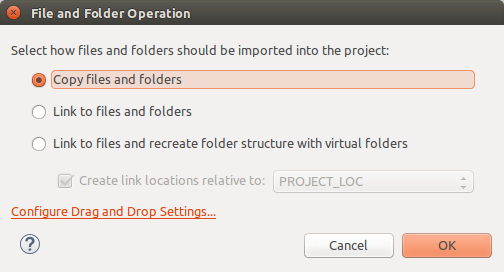
\includegraphics[width=0.8\textwidth] {janelaCopiarLinkar.png}
    \caption{Janela de importação de arquivos}
    \label{fig:janelaCopiarLinkar}
\end{figure}

\subsubsection{Inclusão de caminho na compilação}

Um outro modo de juntar as bibliotecas ao código fonte é adicionando seu caminho à compilação.
Com o projeto selecionado na janela lateral \emph{Project Explorer}, vá em \textbf{Project $>$ Properties $>$ Build $>$ GNU Compiler $>$ Directories} e clique em \emph{Add}, como na figura \ref{fig:incluindoDiretorio}.

\begin{figure}[!h]
\centering
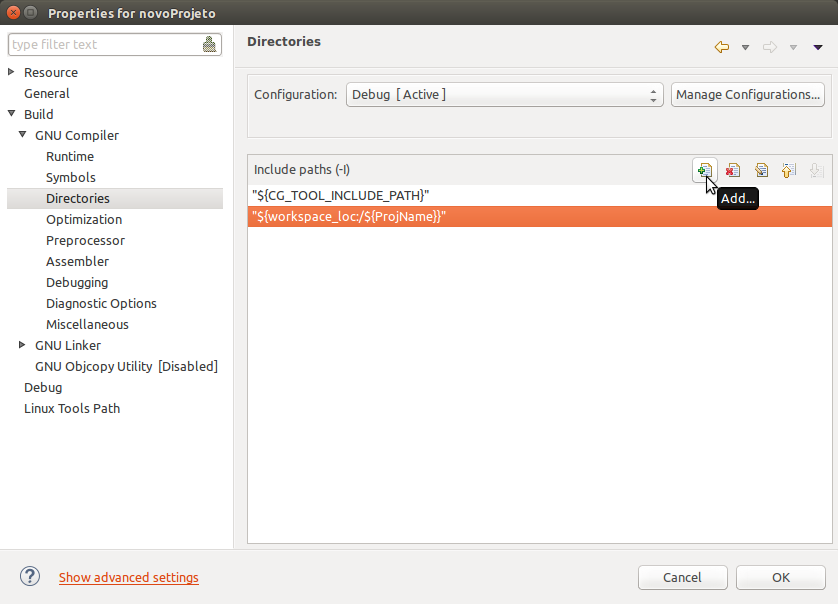
\includegraphics[width=1\textwidth] {incluindoDiretorio.png}
    \caption{Incluindo diretórios para compilação}
    \label{fig:incluindoDiretorio}
\end{figure}

Na janela aberta é possível digitar um caminho para o diretório ou arquivo, mas para prevenir erros existem os botões inferiores que abrirão uma navegação nos diretórios do sistema. Em \textbf{Workspace} é possível escolher o caminho para o diretório de um projeto ou de seus subdiretórios. Em \textbf{Variables} pode-se escolher o caminho armazenado em uma das variáveis de ambiente do projeto. E finalmente, em \textbf{Browse} é possível buscar um diretório navegando pelos arquivos do sistema.

\begin{figure}[H]
\centering
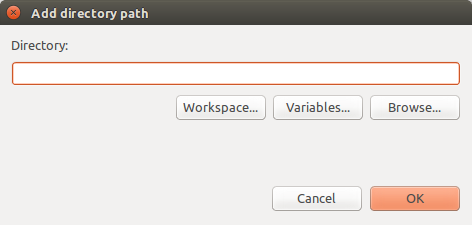
\includegraphics[width=0.8\textwidth] {incluindoDiretorio2.png}
    \caption{Escolhendo diretórios para incluir na compilação}
    \label{fig:incluindoDiretorio2}
\end{figure}

\subsection{TivaWare na ROM}

O TM4C1294NCPDT possui carregado na memória ROM uma parte da biblioteca de drivers do TivaWare. Isso possibilita a geração de um arquivo menor na hora da compilação, economizando memória de programa.

Para o uso das funções gravadas na ROM é necessário importar o arquivo de cabeçalho \emph{'driverlib/rom.h'} e ainda usar o prefixo \emph{'ROM\_'}  junto a função desejada. Por exemplo, para usar a função de configuração de clock do sistema $$SysCtlClockFreqSet()$$ carregada na ROM, esta deve ser chamada como $$ROM\_SysCtlClockFreqSet().$$

Porém, ao chamar tal função da ROM é possível que ela não seja encontrada na hora da compilação. Isso se deve ao fato de que nem todos os hardwares compatíveis com a TivaWare possuem uma memória ROM carregada com sua biblioteca ou mesmo não possua toda ela.
Tal problema é resolvido adicionando-se o arquivo de cabeçalho \emph{'driverlib/rom\_map.h'} e usando o prefixo \emph{'MAP\_'} junto às funções ao invés de \emph{'ROM\_'}. Para o exemplo da função de configuração de clock, a chamada seria feita da forma  $$MAP\_SysCtlClockFreqSet().$$ Esse arquivo de cabeçalho implementa uma estrutura que confere se a função usada existe na ROM do dispositivo para o qual o código será compilado e só assim a substitui. O prefixo de mapeamento pode ser usado em todas as chamadas de funções implementadas pela TivaWare.






\chapter{Sistema de Clock}
Há múltiplas fontes de clock para o uso no microcontrolador. Elas devem ser configuradas logo após um \emph{Power-On Reset} (POR), ou seja, quando o dispositivo é iniciado ou recuperado de um \emph{reset}.

\section{Fontes de clock}
As fontes disponíveis para o controle do TM4C1294NCPDT são:

\begin{description}
	\item [Oscilador Interno de Precisão (\emph{Precision Internal Oscilator}, PIOSC)]\hfill \\
	Fonte de clock interna ao microcontrolador que é usada durante e logo após um POR. É o clock usado para iniciar a execução de uma aplicação. Não necessita de nenhum componente externo e fornece um clock de 16 MHz que apesar de ser preciso varia com temperaturas mais extremas. O PIOSC é útil também para aplicações que não exijam uma fonte de clock tão precisa. Mesmo sendo ou não o clock do sistema, o PIOSC pode ser configurado como fonte de clock de um periférico.
	
	\item [Oscilador Principal (\emph{Main Oscilator}, MOSC)]\hfill \\
	O oscilador principal fornece um clock de precisão por meio de um desses métodos: uma fonte \emph{single-end} de clock é conectada ao pino de entrada OSC0 do microcontrolador, ou um cristal externo é conectado entre o pino de entrada OSC0 e o pino de saída OSC1. Com o PLL em uso, o cristal deve ser de uma frequência entre 5 MHz e 25 MHz. Se não, pode variar de 4 MHz até 25 MHz.
	
	\item [Oscilador Interno de Baixa-frequência (\emph{Low-Frequency Internal Oscillator}, LFIOSC)]\hfill \\
	Clock com frequência nominal de 33 KHz com uma porcentagem de variação. É usado durante os modos de economia de energia \emph{Deep-Sleep}. Estes modos proveem um número reduzido de periféricos em funcionamento e podem desligar o MOSC e/ou PIOSC enquanto o microcontrolador está neste estado.
	
	\item [Oscilador RTC do Módulo de Hibernação (\emph{Hibernation Module RTC Oscillator}, RTCOSC)]\hfill \\
	Fornece uma saída de clock para o sistema selecionável entre duas: um clock externo de 32.768 Hz ou um Clock de Baixa Frequência de Hibernação (HIB LFIOSC). O Módulo de Hibernação pode receber um sinal de clock de 32.768 Hz conectado ao pino XOSC0. O oscilador de 32.768 Hz pode ser usado para o clock do sistema, assim eliminando a necessidade de um cristal ou oscilador adicional. Alternativamente, o Módulo de Hibernação contem um oscilador de baixa frequência (HIB LFIOSC) que provê um RTC para o sistema e pode também prover um clock de precisão para os modos de economia de energia Deep-Sleep ou Hibernação. Note que o HIB LFIOSC é uma fonte de clock diferente de LFIOSC, os dois possuem a mesma frequência nominal mas, enquanto o primeiro pode variar de 10 KHz à 90 KHz, o segundo varia de 10 KHz à 70 KHz.
\end{description}

O clock interno do sistema (SysClk), pode ser derivado de qualquer uma das fontes anteriormente listadas. Um PLL interno pode ser usado pelo PIOSC ou pelo MOSC, e somente estes, para gerar o SysClk e os clocks dos periféricos.

\section{Circuito de verificação do MOSC}

O microcontrolador possui circuitos de controle de clock que verificam se o Oscilador Principal está funcionando adequadamente e na frequência apropriada. O circuito sinaliza quando esta frequência se encontra fora dos valores permitidos para o cristal em uso.

Este circuito deve ser habilitado em tempo de execução. Quando ligado, se um erro for constatado, o MOSC é desligado, é ligado o PIOSC e o sistema é resetado levando o processador a uma interrupção não-mascarável (NMI).


\section{Na TivaWare}

As principais funções de configuração do clock no TivaWare estão listadas abaixo.

\begin{lstlisting}[style=funcao]
	void SysCtlMOSCConfigSet(uint32_t ui32Config)
\end{lstlisting}

Configura o circuito monitor do oscilador principal.

\begin{description}
	\item [\ttbu{ui32Config}]\hfill \\
	Configura o controle do oscilador principal a partir da lógica OR de definições no formato \textbf{SYSCTL\_MOSC\_\emph{k}}, onde \textbf{\emph{k}} pode assumir o valor de:
	\begin{itemize}
		\item \textbf{VALIDATE} para verificar uma falha do MOSC
		\item \textbf{INTERRUPT} quando se deseja gerar uma interrupção ao invés do reset do processador
		\item \textbf{NO\_XTAL} se não há um oscilador esxterno nos pinos OSC0/OSC1, reduzindo o consumo de energia
		\item \textbf{PWR\_DIS} se deseja-se que o MOSC seja desligado. Se este parâmetro não for especificado o oscilador permanece ligado
		\item \textbf{LOWFREQ} se a frequência do MOSC está abaixo de 10 MHZ
		\item \textbf{HIGHFREQ} se a frequência do MOSC está acima de 10 MHZ
		\item \textbf{SESRC} quando o MOSC é um oscilador \emph{single-end} conectado ao pino OSC0. Se não especificado, assume-se que um cristal está em uso.
	\end{itemize}

\end{description}


\begin{lstlisting}[style=funcao]
	uint32_t SysCtlClockFreqSet(uint32_t ui32Config,
								uint32_t ui32SysClock)
\end{lstlisting}

Configura o clock do sistema, frequência de entrada, seu oscilador fonte e o uso ou não do PLL. Retorna o valor da frequência definida em Hz.

\begin{description}
	\item [\ttbu{ui32Config}]\hfill \\
	Configuração do clock. Lógica OR das seguintes máscaras:
	\begin{description}
		\item [SYSCTL\_XTAL\_\emph{k}MHZ] indica o uso de um cristal externo de \textbf{\emph{k}} MHz, podendo assumir os valores: \textbf{5}, \textbf{6}, \textbf{8}, \textbf{10}, \textbf{12}, \textbf{16}, \textbf{18}, \textbf{20}, \textbf{24} ou \textbf{25}.
		
		\item [SYSCTL\_OSC\_\emph{k}] corresponde ao oscilador usado. Sendo \textbf{\emph{k}}:
		\begin{itemize}
			\item \textbf{MAIN} para o oscilador principal
			\item \textbf{INT} para o oscilador interno de precisão de 16 MHz
			\item \textbf{INT30} para o oscilador interno de baixa frequência
			\item \textbf{EXT32} para o oscilador de 32.768 Hz do módulo de hibernação (apenas quando o módulo estiver disponível).
		\end{itemize}
		
		\item [SYSCTL\_USE\_\emph{k}] fonte do clock do sistema. Podendo \textbf{\emph{k}} assumir os valores:
		\begin{itemize}
			\item \textbf{PLL} quando a saída do PLL fornece o clock do sistema.
			\item \textbf{OSC} para o oscilador fonte alimentar o clock do sistema.
		\end{itemize}
		
		\item [SYSCTL\_CFG\_VCO\_\emph{k}] indica a frequência do VCO do PLL quando este está em uso. Os valores de \textbf{\emph{k}} podem somente assumir os valores de \textbf{480} para 480 MHz e \textbf{320} para 320 MHz. O TivaWare escolhe o valor do divisor do PLL para gerar o clock mais próximo do valor desejado a partir destes valores de VCO.
	\end{description}
	
	\item [\ttbu{ui32SysClock}]\hfill \\
	Valor inteiro requerido para o clock do sistema. Se não for possível alcançá-lo com as configurações usadas é assumido o valor mais próximo de clock abaixo deste valor.
\end{description}

\begin{lstlisting}[style=funcao]
	void SysCtlPeripheralEnable(uint32_t ui32Peripheral)
\end{lstlisting}

Habilita o clock em um dos periféricos. Há um período de 5 ciclos de clock da chamada da função até a real ligação do periférico. Cuidados devem ser tomados para que não haja o acesso ao periférico durante este curto espaço de tempo.

\begin{description}
	\item [\ttbu{ui32Peripheral}]\hfill \\
	Periférico a ser ligado o clock.
	\begin{description}
		\item [SYSCTL\_PERIPH\_\emph{k}] indica o periférico à ser habilitado, onde \textbf{\emph{k}} deve ser:
		\begin{itemize}
			\item \textbf{ADC\emph{k}} para representar o AD de número \emph{k}.
			\item \textbf{CAN\emph{k}} para representar o barramento CAN de número \emph{k}.
			\item \textbf{CCM\emph{k}} para representar o módulo CRC do barramento CAN de número \emph{k}.
			\item \textbf{COMP\emph{k}} para representar o comparador de número \emph{k} do AD.
			\item \textbf{EEPROM\emph{k}} para representar a EEPROM de número \emph{k}.
			\item \textbf{EMAC} para representar o módulo Ethernet MAC.
			\item \textbf{EPHY} para representar o módulo Ethernet PHY.
			\item \textbf{EPI} para representar a Interface de Periféricos Externos.
			\item \textbf{GPIO\emph{k}} para representar a GPIO de letra \emph{k}.
			\item \textbf{HIBERNATE} para representar o módulo de hibernação.
			\item \textbf{I2C\emph{k}} para representar o módulo I2C de número \emph{k}.
			\item \textbf{PWM\emph{k}} para representar o módulo de PWM de número \emph{k}.
			\item \textbf{QEI\emph{k}}, \textbf{QEI1} para representar  de número \emph{k}.
			\item \textbf{SSI\emph{k}} para representar o módulo SSI de número \emph{k}.
			\item \textbf{TIMER\emph{k}} para representar o contador de número \emph{k}.
			\item \textbf{UART\emph{k}} para representar o módulo UART de número \emph{k}.
			\item \textbf{UDMA} para representar o módulo de Acesso Direto à Memória.
			\item \textbf{USB\emph{k}} para representar o módulo USB de número \emph{k}.
			\item \textbf{WDOG\emph{k}} para representar o módulo de estouro de tempo de número \emph{k}.
			\item \textbf{WTIMER\emph{k}} para representar o contador do módulo de estouro de tempo de número \emph{k}.
		\end{itemize}

	\end{description}
	
\end{description}

\begin{lstlisting}[style=funcao]
	void SysCtlPeripheralDisable(uint32_t ui32Peripheral)
\end{lstlisting}

Desabilita o clock em um dos periféricos. Uma vez desabilitado, não responderá a nenhum comando.

\begin{description}
	\item [\ttbu{ui32Peripheral}]\hfill \\
	Periférico a ser desabilitado.
	\begin{description}
		\item [SYSCTL\_PERIPH\_\emph{k}] indica o periférico à ser habilitado, onde \textbf{\emph{k}} deve ser:
		\begin{itemize}
			\item \textbf{ADC\emph{k}} para representar o AD de número \emph{k}.
			\item \textbf{CAN\emph{k}} para representar o barramento CAN de número \emph{k}.
			\item \textbf{CCM\emph{k}} para representar o módulo CRC do barramento CAN de número \emph{k}.
			\item \textbf{COMP\emph{k}} para representar o comparador de número \emph{k} do AD.
			\item \textbf{EEPROM\emph{k}} para representar a EEPROM de número \emph{k}.
			\item \textbf{EMAC} para representar o módulo Ethernet MAC.
			\item \textbf{EPHY} para representar o módulo Ethernet PHY.
			\item \textbf{EPI} para representar a Interface de Periféricos Externos.
			\item \textbf{GPIO\emph{k}} para representar a GPIO de letra \emph{k}.
			\item \textbf{HIBERNATE} para representar o módulo de hibernação.
			\item \textbf{I2C\emph{k}} para representar o módulo I2C de número \emph{k}.
			\item \textbf{PWM\emph{k}} para representar o módulo de PWM de número \emph{k}.
			\item \textbf{QEI\emph{k}}, \textbf{QEI1} para representar  de número \emph{k}.
			\item \textbf{SSI\emph{k}} para representar o módulo SSI de número \emph{k}.
			\item \textbf{TIMER\emph{k}} para representar o contador de número \emph{k}.
			\item \textbf{UART\emph{k}} para representar o módulo UART de número \emph{k}.
			\item \textbf{UDMA} para representar o módulo de Acesso Direto à Memória.
			\item \textbf{USB\emph{k}} para representar o módulo USB de número \emph{k}.
			\item \textbf{WDOG\emph{k}} para representar o módulo de estouro de tempo de número \emph{k}.
			\item \textbf{WTIMER\emph{k}} para representar o contador do módulo de estouro de tempo de número \emph{k}.
		\end{itemize}

	\end{description}
	
\end{description}

\begin{lstlisting}[style=funcao]
	void SysCtlPeripheralSleepEnable(uint32_t ui32Peripheral)
\end{lstlisting}

Permite que o periférico continue operando mesmo quando o processador estiver em modo de economia de energia.

\begin{description}
	\item [\ttbu{ui32Peripheral}]\hfill \\
	Periférico a ser habilitado em modo de economia de energia.
	\begin{description}
		\item [SYSCTL\_PERIPH\_\emph{k}] indica o periférico à ser habilitado, onde \textbf{\emph{k}} deve ser:
		\begin{itemize}
			\item \textbf{ADC\emph{k}} para representar o AD de número \emph{k}.
			\item \textbf{CAN\emph{k}} para representar o barramento CAN de número \emph{k}.
			\item \textbf{CCM\emph{k}} para representar o módulo CRC do barramento CAN de número \emph{k}.
			\item \textbf{COMP\emph{k}} para representar o comparador de número \emph{k} do AD.
			\item \textbf{EEPROM\emph{k}} para representar a EEPROM de número \emph{k}.
			\item \textbf{EMAC} para representar o módulo Ethernet MAC.
			\item \textbf{EPHY} para representar o módulo Ethernet PHY.
			\item \textbf{EPI} para representar a Interface de Periféricos Externos.
			\item \textbf{GPIO\emph{k}} para representar a GPIO de letra \emph{k}.
			\item \textbf{HIBERNATE} para representar o módulo de hibernação.
			\item \textbf{I2C\emph{k}} para representar o módulo I2C de número \emph{k}.
			\item \textbf{PWM\emph{k}} para representar o módulo de PWM de número \emph{k}.
			\item \textbf{QEI\emph{k}}, \textbf{QEI1} para representar  de número \emph{k}.
			\item \textbf{SSI\emph{k}} para representar o módulo SSI de número \emph{k}.
			\item \textbf{TIMER\emph{k}} para representar o contador de número \emph{k}.
			\item \textbf{UART\emph{k}} para representar o módulo UART de número \emph{k}.
			\item \textbf{UDMA} para representar o módulo de Acesso Direto à Memória.
			\item \textbf{USB\emph{k}} para representar o módulo USB de número \emph{k}.
			\item \textbf{WDOG\emph{k}} para representar o módulo de estouro de tempo de número \emph{k}.
			\item \textbf{WTIMER\emph{k}} para representar o contador do módulo de estouro de tempo de número \emph{k}.
		\end{itemize}

	\end{description}
	
\end{description}

\begin{lstlisting}[style=funcao]
	void SysCtlPeripheralSleepDisable(uint32_t ui32Peripheral)
\end{lstlisting}

Desabilita o periférico quando o processador estiver em modo de economia de energia. Isso ajuda a diminuir a corrente usada no dispositivo.

\begin{description}
	\item [\ttbu{ui32Peripheral}]\hfill \\
	Periférico a ser desabilitado em modo de economia de energia.
	\begin{description}
		\item [SYSCTL\_PERIPH\_\emph{k}] indica o periférico à ser habilitado, onde \textbf{\emph{k}} deve ser:
		\begin{itemize}
			\item \textbf{ADC\emph{k}} para representar o AD de número \emph{k}.
			\item \textbf{CAN\emph{k}} para representar o barramento CAN de número \emph{k}.
			\item \textbf{CCM\emph{k}} para representar o módulo CRC do barramento CAN de número \emph{k}.
			\item \textbf{COMP\emph{k}} para representar o comparador de número \emph{k} do AD.
			\item \textbf{EEPROM\emph{k}} para representar a EEPROM de número \emph{k}.
			\item \textbf{EMAC} para representar o módulo Ethernet MAC.
			\item \textbf{EPHY} para representar o módulo Ethernet PHY.
			\item \textbf{EPI} para representar a Interface de Periféricos Externos.
			\item \textbf{GPIO\emph{k}} para representar a GPIO de letra \emph{k}.
			\item \textbf{HIBERNATE} para representar o módulo de hibernação.
			\item \textbf{I2C\emph{k}} para representar o módulo I2C de número \emph{k}.
			\item \textbf{PWM\emph{k}} para representar o módulo de PWM de número \emph{k}.
			\item \textbf{QEI\emph{k}}, \textbf{QEI1} para representar  de número \emph{k}.
			\item \textbf{SSI\emph{k}} para representar o módulo SSI de número \emph{k}.
			\item \textbf{TIMER\emph{k}} para representar o contador de número \emph{k}.
			\item \textbf{UART\emph{k}} para representar o módulo UART de número \emph{k}.
			\item \textbf{UDMA} para representar o módulo de Acesso Direto à Memória.
			\item \textbf{USB\emph{k}} para representar o módulo USB de número \emph{k}.
			\item \textbf{WDOG\emph{k}} para representar o módulo de estouro de tempo de número \emph{k}.
			\item \textbf{WTIMER\emph{k}} para representar o contador do módulo de estouro de tempo de número \emph{k}.
		\end{itemize}

	\end{description}
	
\end{description}

\begin{lstlisting}[style=funcao]
	void SysCtlPeripheralClockGating(bool bEnable)
\end{lstlisting}

Habilita e desabilita o clock dos periféricos em modo de economia de energia.

\begin{description}
	\item [\ttbu{bEnable}]\hfill \\
	Valor booleano que deve ser \textbf{true} se os periféricos podem ser usados durante o modo de economia de energia, e \textbf{false} se eles não podem ser usados neste período.
	
\end{description}


\section{Exemplo}

Um exemplo de configuração do clock do microcontrolador é dado a seguir:

\begin{lstlisting}[style=citacao]
// Configurando circuito de verificacao 
// do MOSC para frequencias acima de 10 MHZ
SysCtlMOSCConfigSet(SYSCTL_MOSC_HIGHFREQ);

// Fonte de clock externa de 25 MHz,
// provinda do oscilador principal,
// usando a saida do PLL com fvco = 480 MHz,
// gerando um clock de 120 MHz para o microcontrolador
int systemClockFreq = SysCtlClockFreqSet ( \
			(SYSCTL_XTAL_25MHZ | \
			 SYSCTL_OSC_MAIN | \
			 SYSCTL_USE_PLL | \
			 SYSCTL_CFG_VCO_480), 120000000);

// Habilita o funcionamento da GPIO A e da GPIO B
SysCtlPeripheralEnable(SYSCTL_PERIPH_GPIOA);
SysCtlPeripheralEnable(SYSCTL_PERIPH_GPIOB);

// Habilita o uso somente da GPIO B em 
// modo de economia de energia
// A GPIO A nao podera ser utilizado durante 
// este periodo
SysCtlPeripheralSleepEnable(SYSCTL_PERIPH_GPIOB);

// Habilita o clock nos perifericos em modo de economia de energia
SysCtlPeripheralClockGating(true);

\end{lstlisting}



\chapter{Portas de Entrada e Saída de Propósito Geral (GPIOs)}
O TM4C1294NCPDT possui 15 portas GPIOs de 8 pinos cada. Elas são nomeadas com as letras de \emph{'A'} à \emph{'Q'} menos as letras \emph{'I'} e \emph{'O'}. Algumas das especificações das GPIOs são:

\begin{itemize}
	\item Possui mais de 90 GPIOS, dependendo da configuração usada
	\item Pinos específicos possuem ligação com os periféricos do microcontrolador e suas funções devem ser configuradas
	\item Tensão em configuração de entrada de 3,3 V
	\item Todas as portas são conectadas ao Barramento de Alta Performance (AHB)
	\item Mudança rápida de nível de saída da porta a cada ciclo de clock em portas ligadas ao AHB
	\item Interrupções por pinos nas portas P e Q por bordas de subida, descida ou ambas
	\item Podem ser usadas para iniciar uma sequência de amostragem do A/D ou uma transferência $\mu$DMA
	\item Estado dos pinos podem ser mantidos durante o modo de hibernação; variações de nível nos pinos da porta P podem ser usadas para acordar o sistema da hibernação
	\item Pinos configurados como entradas digital utilizam circuitos Schmitt-trigger
	\item Pinos possuem resistores de pull-up e pull-down e limites de corrente para 2, 4, 6, 8, 10 e 12 mA.
	\item Configuração dreno-aberto habilitada
\end{itemize}




\chapter{Receptor/Transmissor Assíncrono Universal (UART)}
O Transmissor/Receptor Assíncrono Universal (\emph{Universal Asynchronous Receiver/Transmitter}, UART), é um periférico de transmissão e recepção de dados usado na comunicação entre dispositivos, sendo esta comunicação realizada de forma serial e assíncrona, ou seja sem a necessidade de transmissão do sinal de clock de referência. Este modo de transmissão faz necessário o uso de apenas duas vias de comunicação uma para a transmissão e outra para a recepção de dados.

\section{Padrão da Comunicação}

\begin{figure}[H]
\centering
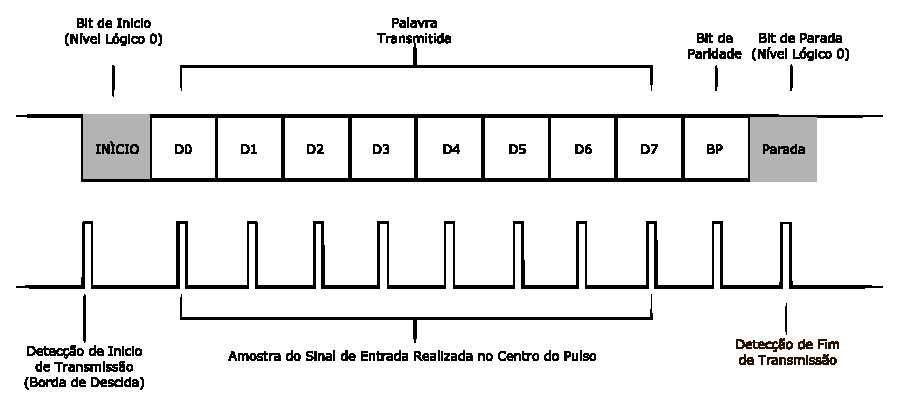
\includegraphics[width=1\textwidth] {figuras/uart.eps}
    \caption{Protocolo de envio na comunicação UART}
    \label{fig:uart}
\end{figure}

Para que a comunicação UART seja realizada é necessário que o sinal de transmissão obedeça a um protocolo. Quando uma palavra é transmitida, primeiro é enviado um bit de início de transmissão para o receptor. Este bit deve ser de nível logico 0 para que a ocorrência da borda de descida sinalize ao receptor que sincronize a amostragem do sinal a ser lido de modo que ela ocorra no meio de cada período de transmissão.  Após transmitir os dados é necessário enviar um bit informando a existência de paridade ou não, e por último é enviado um bit de nível lógico alto para informar o fim da transmissão. Esta sintaxe pode ser observada na figura \ref{fig:uart}.

\section{UART do TM4C1294NCPDT}


O Tiva TM4C1294NCPDT possui 8 módulos de comunicação UART. Cada um destes  possuem um gerador de \emph{baud-rate}, ou taxa de transmissão, que possibilitam  transmissões de até 7,5 Mbps em modo de normal transmissão e  15 Mbps em modo \emph{High Speed}. 

Para que seja possível regular o \emph{baud-rate} de forma mais precisa os módulos UART possuem um divisor de 22 bits, sendo 16 bits inteiros e 6 bits fracionários, pelo qual o módulo determina o período de transmissão de bit.

Já o buffer de leitura e transmissão do UART no Tiva tem um tamanho de 8 bits, porém para cada módulo existe uma FIFO de 16x8 bits tanto para transmissão quanto para recepção, sendo que o \emph{trigger} de interrupção de estouro da FIFO é selecionável entre 1/8, 1/4, 1/2, 3/4, 7/8 ou 8/8. 

O sinal de transmissão criado pelo UART do tiva pode transmitir dados seriais de 5,6,7 ou 8 bits de dados precedidos do bit de \emph{Start} e acompanhados de um bit de paridade, se estiver habilitado, e 1 ou 2 bits de parada. A figura \ref{fig:uartTiva} apresenta o sinal característico da transmissão UART do Tiva. 

\begin{figure}[H]
	\centering
	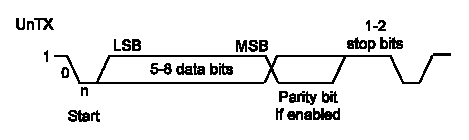
\includegraphics[width=0.5\textwidth] {figuras/uartTiva.eps}
	\caption{Sinal de Transmissão UART no Tiva TM4C1294NCPDT}
	\label{fig:uartTiva}
\end{figure}

A figura \ref{tab:CanaisUART} apresenta os pinos de entrada e saída do UART que podem ser usados no Tiva TM4C1294NCPDT.
  
\begin{table}[H]
	\centering
	\caption{Canais do UART - Tiva TM4C1294NCPDT \cite{DATASHEET_TIVA} }
	\label{tab:CanaisUART}
	\begin{tabular}{|c|c|c|c|l|}
		\rowcolor[HTML]{000000} 
		{\color[HTML]{FFFFFF} Pino}  & {\color[HTML]{FFFFFF} Mux/Função} & {\color[HTML]{FFFFFF} Tipo} & {\color[HTML]{FFFFFF} Buffer} & {\color[HTML]{FFFFFF} Descrição}  \\
		\hline
		UORx  & PA0 (1) & I & TTL & UART Módulo 0, recepção do sinal   \\
		\hline
		U0Tx  & PA1 (1) & O & TTL & UART Módulo 0, transmissão do sinal  \\
		\hline
		\hline
		U1Rx  & PB0 (1) & I & TTL & UART Módulo 1, recepção do sinal   \\
		      & PQ4 (1) &   &     &                                     \\
		\hline
		U1Tx  & PB1 (1) & O & TTL & UART Módulo 1, transmissão do sinal  \\
		\hline
		U2Rx  & PA6 (1) & I & TTL & UART Módulo 2, recepção do sinal   \\
		      & PD4 (1) &   &     &                                      \\
		\hline
		U2Tx  & PA7 (1) & O & TTL & UART Módulo 2, transmissão do sinal  \\
		      & PD5 (1) &   &     &                                      \\
		\hline
		U3Rx  & PA4 (1) (1) & I & TTL & UART Módulo 3, recepção do sinal   \\
	 	      & PJ0 (1) &   &     &                                      \\
		\hline
		U3Tx  & PA5 (1) & O & TTL & UART Módulo 3, transmissão do sinal  \\
	 	      & PJ1 (1) &   &     &                                      \\
		\hline
		U4Rx  & PK0 (1) & I & TTL & UART Módulo 4, recepção do sinal   \\
		      & PA2 (1) &   &     &                                      \\
		\hline
		U4Tx  & PK1 (1) & O & TTL & UART Módulo 4, transmissão do sinal  \\
		      & PA3 (1) &   &     &                                      \\
		\hline
		U5Rx  & PC6 (1) & I & TTL & UART Módulo 5, recepção do sinal\\
		\hline
		U5Tx  & PC7 (1) & O & TTL & UART Módulo 5, transmissão do sinal \\
		\hline
		U6Rx  & PP0 (1) & I & TTL & UART Módulo 6, recepção do sinal \\
		\hline
		U6Tx  & PP1 (1) & O & TTL & UART Módulo 6, transmissão do sinal\\
		\hline
		U7Rx  & PC4 (1) & I & TTL & UART Módulo 7, recepção do sinal \\
		\hline
		U7Tx  & PC5 (1) & O & TTL & UART Módulo 7, transmissão do sinal\\
		\hline
	\end{tabular}
\end{table}


\section{Na TivaWare}

As principais funções para o uso da comunicação UART na TivaWare são apresentadas nesta seção.

\begin{lstlisting}[style=funcao]
	void UARTClockSourceSet(uint32_t ui32Base,
							uint32_t ui32Source);
\end{lstlisting}

Configura a fonte de clock utilizada no barramento UART.

\begin{description}
	\item [\ttbu{ui32Base}]\hfill \\
	Base da UART a ser configurada. Normalmente \textbf{UART\emph{k}\_BASE}, onde \textbf{\emph{k}} é o número que identifica a base que está sendo configurada.
	
	\item [\ttbu{ui32Source}]\hfill \\
	Fonte de clock do UART.
	\begin{description}
		\item [\textbf{UART\_CLOCK\_SYSTEM}] clock fornecido pelo clock do sistema
		\item [\textbf{UART\_CLOCK\_PIOSC}] clock fornecido pelo oscilador interno de precisão
	\end{description}
\end{description}

\begin{lstlisting}[style=funcao]
	void UARTConfigSetExpClk(uint32_t ui32Base,
							 uint32_t ui32UARTClk,
							 uint32_t ui32Baud,
							 uint32_t ui32Config)
\end{lstlisting}

Configura os parâmetros da comunicação UART.

\begin{description}
	\item [\ttbu{ui32Base}]\hfill \\
	Base da UART a ser configurada. Normalmente \textbf{UART\emph{k}\_BASE}, onde \textbf{\emph{k}} é o número que identifica a base que está sendo configurada.
	
	\item [\ttbu{ui32UARTClk}]\hfill \\
	Valor do clock a ser configurado no periférico da UART.
	
	\item [\ttbu{ui32Baud}]\hfill \\
	Baud rate da comunicação UART.
	
	\item [\ttbu{ui32Config}]\hfill \\
	Valor formado pela operação OU lógica de 3 parâmetros: número de bits de dados, número de bits de parada e a paridade.
	
	\begin{description}
		\item [\textbf{UART\_CONFIG\_WLEN\_\emph{k}}] protocolo com \textbf{\emph{k}} bits de dados. Onde \textbf{\emph{k}} pode assumir os valores: 5, 6, 7 e 8
		\item [\textbf{UART\_CONFIG\_STOP\_\emph{k}}] define 1 ou 2 bits de parada. Sendo que \textbf{\emph{k}} assume os valores \textbf{ONE} ou \textbf{TWO}, respectivamente.
		\item [\textbf{UART\_CONFIG\_PAR\_\emph{k}}] onde \textbf{\emph{k}} pode assumir os valores:
		\begin{itemize}
			\item \textbf{NONE} sem bit de paridade
			\item \textbf{EVEN} com bit de paridade par
			\item \textbf{ODD} com bit de paridade ímpar
			\item \textbf{ONE} bit de paridade é sempre 1
			\item \textbf{ZERO} bit de paridade é sempre 0
		\end{itemize}

	\end{description}
\end{description}

\begin{lstlisting}[style=funcao]
	void UARTEnable(uint32_t ui32Base)
\end{lstlisting}

Habilita o funcionamento da comunicação UART.

\begin{description}
	\item [\ttbu{ui32Base}]\hfill \\
	Base da UART a ser habilitada. Normalmente \textbf{UART\emph{k}\_BASE}, onde \textbf{\emph{k}} é o número que identifica a base que está sendo configurada.
\end{description}

\begin{lstlisting}[style=funcao]
	void UARTDisable(uint32_t ui32Base)
\end{lstlisting}

Desabilita o funcionamento da comunicação UART.

\begin{description}
	\item [\ttbu{ui32Base}]\hfill \\
	Base da UART a ser desabilitada. Normalmente \textbf{UART\emph{k}\_BASE}, onde \textbf{\emph{k}} é o número que identifica a base que está sendo configurada.
\end{description}

\begin{lstlisting}[style=funcao]
	int32_t UARTCharGet(uint32_t ui32Base)
\end{lstlisting}

Pega próximo caractere recebido pela UART. Se não houver nada para ser lido, o programa trava e espera até haver um caractere.

\begin{description}
	\item [\ttbu{ui32Base}]\hfill \\
	Base da UART a ser lida. Normalmente \textbf{UART\emph{k}\_BASE}, onde \textbf{\emph{k}} é o número que identifica a base que está sendo configurada.
\end{description}

\begin{lstlisting}[style=funcao]
	int32_t UARTCharGetNonBlocking(uint32_t ui32Base)
\end{lstlisting}

Pega próximo caractere recebido pela UART. Se não houver nada para ser lido, a leitura é ignorada e o programa continua normalmente. Nesse caso, a função retorna -1.

\begin{description}
	\item [\ttbu{ui32Base}]\hfill \\
	Base da UART a ser lida. Normalmente \textbf{UART\emph{k}\_BASE}, onde \textbf{\emph{k}} é o número que identifica a base que está sendo configurada.
\end{description}

\begin{lstlisting}[style=funcao]
	void UARTCharPut(uint32_t ui32Base,
					 unsigned char ucData))
\end{lstlisting}

Envia um caractere para ser transmitido pela UART. Se não houver espaço na fila de transmissão, o programa é travado e aguarda até o caractere ser colocado na fila.

\begin{description}
	\item [\ttbu{ui32Base}]\hfill \\
	Base da UART a ser lida. Normalmente \textbf{UART\emph{k}\_BASE}, onde \textbf{\emph{k}} é o número que identifica a base que está sendo configurada.
	
	\item [\ttbu{ucData}]\hfill \\
	Caractere a ser transmitido pela UART.
\end{description}

\begin{lstlisting}[style=funcao]
	bool UARTCharPutNonBlocking(uint32_t ui32Base,
								unsigned char ucData))
\end{lstlisting}

Envia um caractere para ser transmitido pela UART. Se não houver espaço na fila de transmissão, a operação é ignorada e o programa continua normalmente. Nesse caso, a função retorna o valor \emph{false} e a operação deve ser repetida posteriormente.

\begin{description}
	\item [\ttbu{ui32Base}]\hfill \\
	Base da UART a ser lida. Normalmente \textbf{UART\emph{k}\_BASE}, onde \textbf{\emph{k}} é o número que identifica a base que está sendo configurada.
	
	\item [\ttbu{ucData}]\hfill \\
	Caractere a ser transmitido pela UART.
\end{description}

\begin{lstlisting}[style=funcao]
	bool UARTCharsAvail(uint32_t ui32Base)
\end{lstlisting}

Informa se há algum caractere para ser lido na fila de recepção.

\begin{description}
	\item [\ttbu{ui32Base}]\hfill \\
	Base da UART a ser lida. Normalmente \textbf{UART\emph{k}\_BASE}, onde \textbf{\emph{k}} é o número que identifica a base que está sendo configurada.
\end{description}

\begin{lstlisting}[style=funcao]
	bool UARTSpaceAvail(uint32_t ui32Base)
\end{lstlisting}

Informa se há espaço para ser enviado um novo byte para a fila de transmissão.

\begin{description}
	\item [\ttbu{ui32Base}]\hfill \\
	Base da UART a ser lida. Normalmente \textbf{UART\emph{k}\_BASE}, onde \textbf{\emph{k}} é o número que identifica a base que está sendo configurada.
\end{description}

\begin{lstlisting}[style=funcao]
	void UARTIntRegister(uint32_t ui32Port,
						 void (*pfnIntHandler)(void))
\end{lstlisting}

Configura a função de tratamento de uma interrupção da UART. Aquela que é chamada quando ocorre a interrupção.

\begin{description}
	\item [\ttbu{ui32Base}]\hfill \\
	Base da UART a ser configurada. Normalmente \textbf{UART\emph{k}\_BASE}, onde \textbf{\emph{k}} é o número que identifica a base que está sendo configurada.
	
	\item [\ttbu{pfnIntHandler}]\hfill \\
	Ponteiro da função de tratamento. Esta não deve receber nada como parâmetro e nem retornar nada.
\end{description}

\begin{lstlisting}[style=funcao]
	void UARTIntEnable(uint32_t ui32Base,
					   uint32_t ui32IntFlags)
\end{lstlisting}

Habilita as interrupções especificadas da UART especificada.

\begin{description}
	\item [\ttbu{ui32Base}]\hfill \\
	Base da UART a ser configurada. Normalmente \textbf{UART\emph{k}\_BASE}, onde \textbf{\emph{k}} é o número que identifica a base que está sendo configurada.
	
	\item [\ttbu{ui32IntFlags}]\hfill \\
	Pacote em formato de OU lógico com os parâmetros que especificam os eventos que podem causar a interrupção da UART. Cada parâmetro recebe uma definição no formato \textbf{UART\_INT\_\emph{k}}, onde \textbf{\emph{k}} é um valor entre os seguintes:
	\begin{itemize}
		\item \textbf{9BIT} interrupção por endereço de 9 bits
		\item \textbf{OE} interrupção por transbordo de fila
		\item \textbf{BE} interrupção por erro de parada
		\item \textbf{PE} interrupção por erro de paridade
		\item \textbf{FE} interrupção por erro de enquadramento
		\item \textbf{RT} interrupção por estouro de tempo de recepção
		\item \textbf{TX} interrupção por transmissão
		\item \textbf{RX} interrupção por recepção
		\item \textbf{DSR} interrupção por DSR
		\item \textbf{DCD} interrupção por DCD
		\item \textbf{CTS} interrupção por CTS
		\item \textbf{RI} interrupção por RI
	\end{itemize}
\end{description}

\begin{lstlisting}[style=funcao]
	void UARTIntDisable(uint32_t ui32Base,
					   uint32_t ui32IntFlags)
\end{lstlisting}

Desabilita as interrupções especificadas da UART especificada.

\begin{description}
	\item [\ttbu{ui32Base}]\hfill \\
	Base da UART a ser configurada. Normalmente \textbf{UART\emph{k}\_BASE}, onde \textbf{\emph{k}} é o número que identifica a base que está sendo configurada.
	
	\item [\ttbu{ui32IntFlags}]\hfill \\
	Pacote em formato de OU lógico com os parâmetros que especificam os eventos que podem causar a interrupção da UART. Cada parâmetro recebe uma definição no formato \textbf{UART\_INT\_\emph{k}}, onde \textbf{\emph{k}} é um valor entre os seguintes:
	\begin{itemize}
		\item \textbf{9BIT} interrupção por endereço de 9 bits
		\item \textbf{OE} interrupção por transbordo de fila
		\item \textbf{BE} interrupção por erro de parada
		\item \textbf{PE} interrupção por erro de paridade
		\item \textbf{FE} interrupção por erro de enquadramento
		\item \textbf{RT} interrupção por estouro de tempo de recepção
		\item \textbf{TX} interrupção por transmissão
		\item \textbf{RX} interrupção por recepção
		\item \textbf{DSR} interrupção por DSR
		\item \textbf{DCD} interrupção por DCD
		\item \textbf{CTS} interrupção por CTS
		\item \textbf{RI} interrupção por RI
	\end{itemize}
\end{description}

\begin{lstlisting}[style=funcao]
	void UARTIntClear(uint32_t ui32Base,
					   uint32_t ui32IntFlags)
\end{lstlisting}

Limpa a flag que armazena a ocorrência das interrupções especificadas da UART especificada.

\begin{description}
	\item [\ttbu{ui32Base}]\hfill \\
	Base da UART a ser configurada. Normalmente \textbf{UART\emph{k}\_BASE}, onde \textbf{\emph{k}} é o número que identifica a base que está sendo configurada.
	
	\item [\ttbu{ui32IntFlags}]\hfill \\
	Pacote em formato de OU lógico com os parâmetros que especificam as interrupção da UART a serem limpas. Cada parâmetro recebe uma definição no formato \textbf{UART\_INT\_\emph{k}}, onde \textbf{\emph{k}} é um valor entre os seguintes:
	\begin{itemize}
		\item \textbf{9BIT} interrupção por endereço de 9 bits
		\item \textbf{OE} interrupção por transbordo de fila
		\item \textbf{BE} interrupção por erro de parada
		\item \textbf{PE} interrupção por erro de paridade
		\item \textbf{FE} interrupção por erro de enquadramento
		\item \textbf{RT} interrupção por estouro de tempo de recepção
		\item \textbf{TX} interrupção por transmissão
		\item \textbf{RX} interrupção por recepção
		\item \textbf{DSR} interrupção por DSR
		\item \textbf{DCD} interrupção por DCD
		\item \textbf{CTS} interrupção por CTS
		\item \textbf{RI} interrupção por RI
	\end{itemize}
\end{description}

\section{Exemplo}

A seguir, é apresentado um exemplo de configuração da UART. Um exemplo mais abrangente pode ser visto na Seção \ref{sec:exUart}

\begin{lstlisting}[style=citacao]
	// Habilita GPIO A usado na comunicacao da UART 0
	MAP_SysCtlPeripheralEnable(SYSCTL_PERIPH_GPIOA);
	// Aguarda 3 SysCtlDelay
	// Aproximadamente 10 ciclos de clock
	MAP_SysCtlDelay(3);
	// Configura PA0 no modo Rx da UART 0
	MAP_GPIOPinConfigure(GPIO_PA0_U0RX);
	// Configura PA1 no modo Tx da UART 0
	MAP_GPIOPinConfigure(GPIO_PA1_U0TX);

	// Habilita UART 0
	MAP_SysCtlPeripheralEnable(SYSCTL_PERIPH_UART0);
	// Configura PA0 e PA1 como pinos de comunicacao da UART
	MAP_GPIOPinTypeUART(
		GPIO_PORTA_BASE, GPIO_PIN_0 | GPIO_PIN_1);
	// Configura UART 0
	// fonte de clock 120MHz para 115.200 baud 8N1
	UARTConfigSetExpClk(UART0_BASE, 120000000, 115200,
		(UART_CONFIG_WLEN_8 | UART_CONFIG_STOP_ONE | 
		UART_CONFIG_PAR_NONE));

	// Configura rotina de tratamento de interrupcao da UART
	UARTIntRegister(UART0_BASE, UARTIntHandler);
	// Habilita interrupcao da UART 0
	MAP_IntEnable(INT_UART0);
	// Configura pinos de interrupcao da UART 0
	MAP_UARTIntEnable(UART0_BASE, UART_INT_RX | UART_INT_RT);
\end{lstlisting}




\chapter{Barramento SPI}
A Interface de Periféricos Serial, ou SPI (\emph{Serial Peripheral Interface}) é dispositivo usado para a transmissão e recepção serial de dados. Sendo uma comunicação síncrona, a SPI necessita de uma fonte de clock de referência para se estabelecer, além de um sinal de \emph{chip select}, ou \textbf{CS}, para ativar a recepção de dados no dispositivo receptor. Deste modo esta comunicação requer no minimo três vias de transmissão, sendo que a comunicação em cada barramento é unidirecional.

\section{Padrão da Comunicação}

A comunicação SPI possui a maior taxa de transmissão, ou \emph{baud-rate}, dentre os demais protocolos de comunicação usados em microcontroladores, podendo chegar a até a 66Mpbs em periféricos com o AT45BD0100D da Adesto. O que possibilita um  \emph{baud-rate} tão elevado é o fato de que nesta comunicação a recepção e a transmissão de dados é feita separadamente e de forma direta, sem a necessidade de se transmitir bits de inicio ou termino de transmissão, e ainda de modo que o controle da transmissão é realizado pelo sinal CS (Chip Select) e pelo sinal  CLK (Clock).  A figura \ref{fig:SPI} apresenta o padrão de uma comunicação SPI.

\begin{figure}[H]
	\centering
	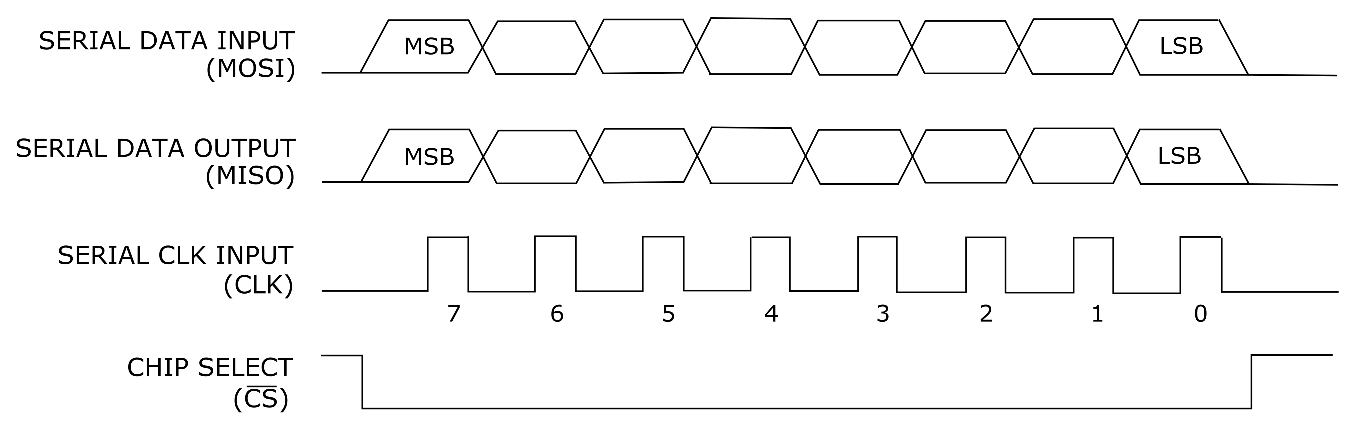
\includegraphics[width=1\textwidth] {figuras/PadraoSPI.eps}
	\caption{Padrão de Comunicação SPI}
	\label{fig:SPI}
\end{figure}

Para transmitir um dado de um dispositivo \textbf{Mestre} para um \textbf{Escravo} é necessário que o \textbf{Mestre} ative o sinal de CS do \textbf{Escravo} e forneça a ele o sinal de clock de referência. Em seguida bit a bit deve ser transmitido pela porta MOSI \emph{Master Output - Slave Input} de ambos os dispositivos. 

Quando for necessário transmitir um dado de um  \textbf{Escravo} para um \textbf{Mestre}, novamente o \textbf{Mestre} deve ativar o sinal de CS do  \textbf{Escravo} e fornecer a ele o sinal de clock de referência, porém o dado será transmitido bit a bit pela porta MISO \emph{Master Input - Slave Output} de ambos os dispositivos. 

\begin{figure}[H]
	\centering
	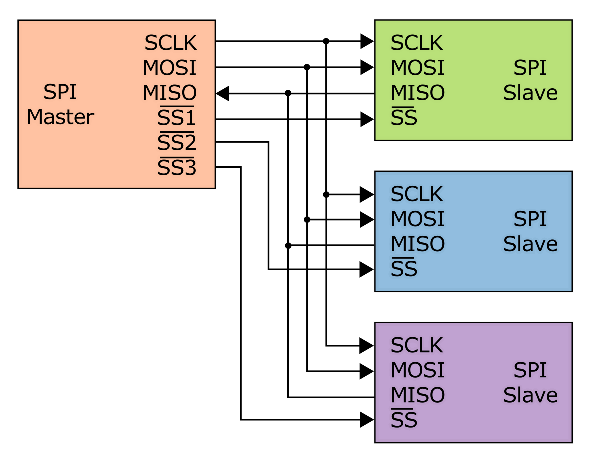
\includegraphics[width=0.6\textwidth] {figuras/BarramentoSPI.eps}
	\caption{Diagrama de Comunicação SPI - Vários Escravos}
	\label{fig:SPIDiagrama}
\end{figure}

A figura  \ref{fig:SPIDiagrama} apresenta um diagrama básico de uma comunicação entre \textbf{Mestre} e vários \textbf{Escravos} através dos barramentos de dados e de clock em comum.  

\section{SPI do TM4C1294NCPDT}

No Tiva - TM4C1294NCPDT a comunicação SPI se dá através do Interface Serial Quad Sincrona (\emph{Quad Synchronous Serial Interface}), ou QSSI. Há 4 módulos QSSI no Tiva, todos capazes de transmitir dados no modo Advanced, Bi-SSI e Quad-SSI.

No modo de transmissão Bi-SSI, dois pinos de dados são ativados para receber ou transmitir; SSInXDAT0 e o SSInXDAT1. Já no modo de transmissão Quad-SSI, quatro pinos são ativados para receber ou transmitir dados; SSInXDAT0, SSInXDAT1, SSInXDAT2 e SSInXDAT4. 

No modo de transmissão Advanced, a transmissão se realiza de modo que ao transmitir um dado por um pino, o outro pino fica impossibilitado de receber, e vice-versa.

A forma de transmissão dos módulos QSSI podem ser alterados entre os formatos \emph{Texas Instruments synchronous serial} e \emph{Freescale SPI}. Logo para transmitir em modo SPI basta somente selecionar o modo \emph{Freescale SPI}, podendo utilizar tanto o modo de transmissão Bi- ou  Quad-SSI.

No modo de comunicação SPI, tem-se um \emph{baud rate} máximo de 2MHz e uma FIFO para transmissão e outra para recepção ambas com capacidade de 16x8 bits. É possível alternar a fonte de clock de referência da transmissão entre o clock padrão do sistema (SYSCLK) e o clock alternativo (ALTCLK), contando ainda com um divisor de clock de 8 bits, que possibilita dividir o clock de 1 até 254 vezes.  

Como é comum na comunicação SPI o Tiva possui portas para transmissão, recepção e clock exclusiva para cada  módulo de comunicação. A tabela \ref{tab:CanaisSPI} apresenta as referidas portas para comunicação SPI.

\begin{table}[H]
	\centering
	\caption{Canais do SPI - Tiva TM4C1294NCPDT \cite{DATASHEET_TIVA} }
	\label{tab:CanaisSPI}
	\begin{tabular}{|c|c|c|c|l|}
		\rowcolor[HTML]{000000} 
		{\color[HTML]{FFFFFF} Pino}  & {\color[HTML]{FFFFFF} Mux/Função} & {\color[HTML]{FFFFFF} Tipo} & {\color[HTML]{FFFFFF} Buffer} & {\color[HTML]{FFFFFF} Descrição}  \\
		\hline
		SSI0CLK   & PA2 (15) & I/O & TTL & SPI Módulo 0, sinal de clock   \\
		\hline
		SSI0XDAT0 & PA4 (15) & I/O & TTL & SPI Módulo 0, MISO \\
		\hline
		SSI0XDAT1 & PA5 (15) & I/O & TTL & SPI Módulo 0, MOSI \\
		\hline
		SSI1CLK   & PB5 (15) & I/O & TTL & SPI Módulo 1, sinal de clock   \\
		\hline
		SSI1XDAT0 & PE4 (15) & I/O & TTL & SPI Módulo 1, MISO  \\
		\hline
		SSI1XDAT1 & PE5 (15) & I/O & TTL & SPI Módulo 1, MOSI  \\
		\hline
		SSI2CLK   & PB5 (15) & I/O & TTL & SPI Módulo 2, sinal de clock   \\
		\hline
		SSI2XDAT0 & PD1 (15) & I/O & TTL & SPI Módulo 2, MISO  \\
		\hline
		SSI2XDAT1 & PD0 (15) & I/O & TTL & SPI Módulo 2, MOSI  \\
		\hline
		SSI3CLK   & PQ0 (14) & I/O & TTL & SPI Módulo 3, sinal de clock   \\
		          & PF3 (14) &     &     &                                \\
		\hline
		SSI3XDAT0 & PQ2 (14) & I/O & TTL & SPI Módulo 3, MISO  \\
		          & PF1 (14) &     &     &                     \\
		\hline
		SSI3XDAT1 & PQ3 (14) & I/O & TTL & SPI Módulo 3, MOSI  \\
		          & PF0 (14) &     &     &                     \\
		\hline
	\end{tabular}
\end{table}


\section{SPI Na TivaWare}

\section{Exemplo}

\chapter{Conversor Analógico/Digital ADC}
O ADC (\emph{Analog-To-Digital Converter}) é um periférico responsável por realizar a conversão de uma grandeza analógica de tensão para um valor correspondente digital. Para realizar esta conversão pode-se implementar vários  tipos circuito, como o conversor flash, ou o conversor de aproximações sucessivas, ou ainda conversor integrador simples ou de rampa dupla. Porém o  circuito de conversão mais usado em circuito integrados atualmente é o conversor de aproximações sucessivas, o qual também usado como AD no Tiva TM4C1294NCPDT. 


\section{ADC de Aproximações Sucessivas}

\begin{figure}[H]
	\centering
	\fbox{
	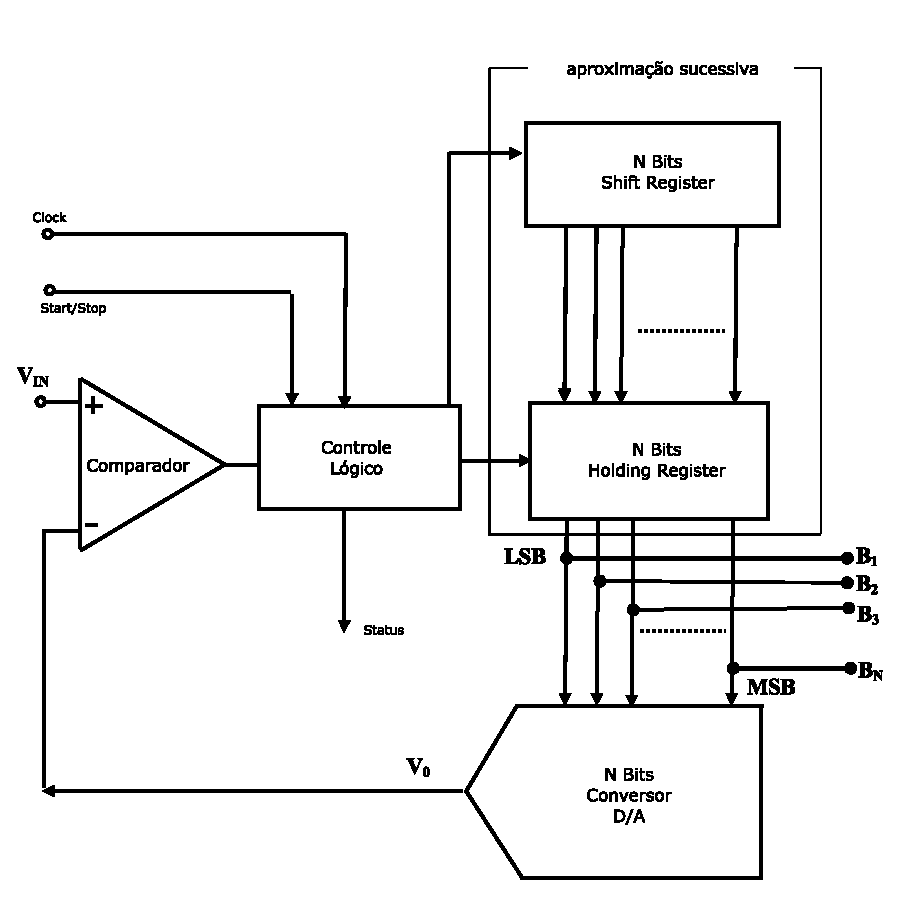
\includegraphics[width=0.5\textwidth] {figuras/ConversorAD.eps}}
	\caption{Conversor A/D tipo Aproximação Sucessiva}
	\label{fig:ConversorAD}
\end{figure}

 A figura \ref{fig:ConversorAD} apresenta o diagrama básico de funcionamento de um conversor de aproximações sucessivas. Nota-se que tal conversor utiliza a técnica de realimentação para relacionar uma voltagem analógica de entrada com um código digital, através de um conversor DA (\emph{Digital-To-Analog Converter}) e um comparador. O processo de conversão inicia quando o \emph{Shift Register} e o \emph{Holding Register} são zerados, e então o MSB (\emph{Most Significant Bit}) do \emph{Holding Register} vai para nível alto. Em seguida o comparador relaciona a saída do conversor DA com a tensão $V_{IN}$. Se $V_{O} < V_{IN}$ a conversão chega ao fim, porém se isso não for verdade a etapa se repete e MSB vai para nível baixo e o segundo SB vai para nível alto. E assim se dá a conversão. 

\section{ADC do TM4C1294NCPDT}

O Tiva TM4C1294NCPDT possui 2 módulos de conversão AD  de 12-bit, que podem ser usados em qualquer um das 20 entradas de sinal analógico. É possível realizar amostragens sequenciais entre os canais ou no mesmo canal repetidamente com intervalos de tempo  programáveis. Cada módulo AD possui 8 comparadores que possibilitam realizar comparações entre os sinais de entrada e  valores pré-definidos, para que assim possa ser realizado as mais diversas operações.  Ainda é possível usar um \emph{trigger} diferente para cada um dos módulos, ou usar um \emph{trigger} para acionar ambos os módulos.

A tabela \ref{tab:CanaisADC} apresenta os pinos de entrada para os módulos ADC0 e ADC1, com a descrição do nome do pino de entrada, o numero referente a este pino, sua função e o tipo de \emph{buffer} usado. Nesta mesma tabela temos o  pino chamado de $VREFA+$ que é o pino da tensão de referência usado pelo AD. A $VREFA+$ corresponde o valor máximo que o conversor DA, usado pelo AD para realizar a comparação com a tensão de entrada, pode atingir. 

A tensão $VREFA+$ é extremamente importante para se realizar a conversão AD, pois se este valor não for selecionado de forma adequada pode-se acarretar problemas no valor digital. A tensão $VREFA+$ pode ser alternada entre uma fonte de referência interna ou externa. 

\begin{center}
\begin{longtable}{|c|c|c|c|c|c|}
	\rowcolor[HTML]{000000}
	{\color[HTML]{FFFFFF} Pino} & {\color[HTML]{FFFFFF} $n^{o}$} & {\color[HTML]{FFFFFF} Mux/Função} & {\color[HTML]{FFFFFF} Tipo} & {\color[HTML]{FFFFFF} Buffer} & {\color[HTML]{FFFFFF} Descrição}            \\
	AIN0                        & 12                             & PE3                               & I                           & Analógico                     & ADC - Entrada 0                             \\
	\hline
	AIN1                        & 13                             & PE2                               & I                           & Analógico                     & ADC - Entrada 1                             \\
	\hline
	AIN2                        & 14                             & PE1                               & I                           & Analógico                     & ADC - Entrada 2                             \\
	\hline
	AIN3                        & 15                             & PE0                               & I                           & Analógico                     & ADC - Entrada 3                             \\
	\hline
	AIN4                        & 128                            & PD7                               & I                           & Analógico                     & ADC - Entrada 4                             \\
	\hline
	AIN5                        & 127                            & PD6                               & I                           & Analógico                     & ADC - Entrada 5                             \\
	\hline
	AIN6                        & 126                            & PD5                               & I                           & Analógico                     & ADC - Entrada 6                             \\
	\hline
	AIN7                        & 125                            & PD4                               & I                           & Analógico                     & ADC - Entrada 7                             \\
	\hline
	AIN8                        & 124                            & PE5                               & I                           & Analógico                     & ADC - Entrada 8                             \\
	\hline
	AIN9                        & 123                            & PE4                               & I                           & Analógico                     & ADC - Entrada 9                             \\
	\hline
	AIN10                       & 121                            & PB4                               & I                           & Analógico                     & ADC - Entrada 10                            \\
	\hline
	AIN11                       & 120                            & PB5                               & I                           & Analógico                     & ADC - Entrada 11                            \\
	\hline
	AIN12                       & 4                              & PD3                               & I                           & Analógico                     & ADC - Entrada 12                            \\
	\hline
	AIN13                       & 3                              & PD2                               & I                           & Analógico                     & ADC - Entrada 13                            \\
	\hline
	AIN14                       & 2                              & PD1                               & I                           & Analógico                     & ADC - Entrada 14                            \\
	\hline
	AIN15                       & 1                              & PD0                               & I                           & Analógico                     & ADC - Entrada 15                            \\
	\hline
	AIN16                       & 18                             & PK0                               & I                           & Analógico                     & ADC - Entrada 16                            \\
	\hline
	AIN17                       & 19                             & PK1                               & I                           & Analógico                     & ADC - Entrada 17                            \\
	\hline
	AIN18                       & 20                             & PK2                               & I                           & Analógico                     & ADC - Entrada 18                            \\
	\hline
	AIN19                       & 21                             & PK3                               & I                           & Analógico                     & ADC - Entrada 19                            \\
	\hline
	&                                &                                   &                             &                               & A tensão de referência                      \\
	&                                &                                   &                             &                               & \multicolumn{1}{l|}{é usada pelo AD para}    \\
	&                                &                                   &                             &                               & \multicolumn{1}{l|}{fixar o valor máximo de} \\
	\multirow{-4}{*}{VREFA+}    & \multirow{-4}{*}{9}            & \multirow{-4}{*}{fixo}            & \multirow{-4}{*}{-}         & \multirow{-4}{*}{Analógico}   & \multicolumn{1}{l|}{conversão.}  \\ 
	\hline
	\caption{Canais de Entrada ADC - Tiva TM4C1294NCPDT \cite{DATASHEET_TIVA} }
	\label{tab:CanaisADC}
\end{longtable}
\end{center}

\section{Na TivaWare}

As principais funções, da biblioteca TivaWare, responsáveis pela configuração e utilização do ADC, são listadas a seguir.

\begin{lstlisting}[style=funcao]
	void ADCSequenceConfigure(uint32_t ui32Base,
							  uint32_t ui32SequenceNum,
							  uint32_t ui32Trigger,
							  uint32_t ui32Priority)
\end{lstlisting}

Configurações básicas do ADC especificado.

\begin{description}
	\item [\ttbu{ui32Base}]\hfill \\
	Base do ADC a ser configurado. Normalmente \textbf{ADC\emph{k}\_BASE}, onde \textbf{\emph{k}} é a letra identificadora do periférico.
	
	\item [\ttbu{ui32SequenceNum}]\hfill \\
	Número da sequência de amostragem.
	
	\item [\ttbu{ui32Trigger}]\hfill \\
	Evento que aciona o amostrador. Definido no formato \textbf{ADC\_TRIGGER\_\emph{k}}, onde \textbf{\emph{k}} pode assumir um dos valores:
	\begin{itemize}
		\item \textbf{PROCESSOR} amostragem iniciada por comando de software.
		\item \textbf{COMP0} amostragem iniciada pelo comparador 0 do ADC.
		\item \textbf{COMP1} amostragem iniciada pelo comparador 1 do ADC.
		\item \textbf{COMP2} amostragem iniciada pelo comparador 2 do ADC.
		\item \textbf{EXTERNAL} amostragem iniciada por uma GPIO de entrada configurada.
		\item \textbf{TIMER} amostragem iniciada pelo temporizador.
		\item \textbf{PWM0} amostragem iniciada pelo PWM 0.
		\item \textbf{PWM1} amostragem iniciada pelo PWM 1.
		\item \textbf{PWM2} amostragem iniciada pelo PWM 2.
		\item \textbf{PWM3} amostragem iniciada pelo PWM 3.
		\item \textbf{ALWAYS} amostragem iniciada repetida e continuamente
	\end{itemize}
\end{description}

\begin{lstlisting}[style=funcao]
	void ADCSequenceStepConfigure(uint32_t ui32Base,
								  uint32_t ui32SequenceNum,
								  uint32_t ui32Step,
								  uint32_t ui32Config)
\end{lstlisting}

Configura o intervalo de amostragem do ADC especificado.

\begin{description}
	\item [\ttbu{ui32Base}]\hfill \\
	Base do ADC a ser configurado. Normalmente \textbf{ADC\emph{k}\_BASE}, onde \textbf{\emph{k}} é a letra identificadora do periférico.
	
	\item [\ttbu{ui32SequenceNum}]\hfill \\
	Número da sequência de amostragem.
	
	\item [\ttbu{ui32Step}]\hfill \\
	Intervalo de amostragem do ADC.
	
	\item [\ttbu{ui32Config}]\hfill \\
	Configuração da amostragem. Pacote de OU lógico de valores no formato \textbf{ADC\_CTL\_\emph{k}}, onde \textbf{\emph{k}} pode assumir os valores:
	\begin{itemize}
		\item \textbf{TS} amostragem do sensor de temperatura interno.
		\item \textbf{IE} amostragem gera interrupção.
		\item \textbf{END} amostragem por sequencia e seleção.
		\item \textbf{D} amostragem por seleção diferencial.
		\item \textbf{CH\emph{k}} seleciona canal de entrada como canal \textbf{\emph{k}}, onde \textbf{\emph{k}} assume valores de 0 a 23.
		\item \textbf{CMP\emph{k}} seleciona comparador \textbf{\emph{k}} para ser utilizado, onde \textbf{\emph{k}} assume valores de 0 a 7.
	\end{itemize}
\end{description}

\begin{lstlisting}[style=funcao]
	void ADCSequenceEnable(uint32_t ui32Base,
						   uint32_t ui32SequenceNum)
\end{lstlisting}

Habilita a sequência de amostragem.

\begin{description}
	\item [\ttbu{ui32Base}]\hfill \\
	Base do ADC a ser configurado. Normalmente \textbf{ADC\emph{k}\_BASE}, onde \textbf{\emph{k}} é a letra identificadora do periférico.
	
	\item [\ttbu{ui32SequenceNum}]\hfill \\
	Número da sequência de amostragem.
\end{description}

\begin{lstlisting}[style=funcao]
	void ADCSequenceDisable(uint32_t ui32Base,
							uint32_t ui32SequenceNum)
\end{lstlisting}

Desabilita a sequência de amostragem.

\begin{description}
	\item [\ttbu{ui32Base}]\hfill \\
	Base do ADC a ser configurado. Normalmente \textbf{ADC\emph{k}\_BASE}, onde \textbf{\emph{k}} é a letra identificadora do periférico.
	
	\item [\ttbu{ui32SequenceNum}]\hfill \\
	Número da sequência de amostragem.
\end{description}

\begin{lstlisting}[style=funcao]
	int32_t ADCSequenceDataGet(uint32_t ui32Base,
							   uint32_t ui32SequenceNum,
							   uint32_t *pui32Buffer)
\end{lstlisting}

Pega o valor gerado na amostragem.

\begin{description}
	\item [\ttbu{ui32Base}]\hfill \\
	Base do ADC a ser lido. Normalmente \textbf{ADC\emph{k}\_BASE}, onde \textbf{\emph{k}} é a letra identificadora do periférico.
	
	\item [\ttbu{ui32SequenceNum}]\hfill \\
	Número da sequência de amostragem.
	
	\item [\ttbu{pui32Buffer}]\hfill \\
	Ponteiro para uma região de memória alocada. Onde será armazenado o valor lido.
\end{description}

\begin{lstlisting}[style=funcao]
	int32_t ADCSequenceDataGet(uint32_t ui32Base,
							   uint32_t ui32SequenceNum,
							   uint32_t *pui32Buffer)
\end{lstlisting}

Pega o valor gerado na amostragem.

\begin{description}
	\item [\ttbu{ui32Base}]\hfill \\
	Base do ADC a ser lido. Normalmente \textbf{ADC\emph{k}\_BASE}, onde \textbf{\emph{k}} é a letra identificadora do periférico.
	
	\item [\ttbu{ui32SequenceNum}]\hfill \\
	Número da sequência de amostragem.
	
	\item [\ttbu{pui32Buffer}]\hfill \\
	Ponteiro para uma região de memória alocada. Onde será armazenado o valor lido.
\end{description}

\begin{lstlisting}[style=funcao]
	int32_t ADCSequenceOverflow(uint32_t ui32Base,
								uint32_t ui32SequenceNum)
\end{lstlisting}

Informa se houve uma perda de leitura, antes de ter lido o valor antigo ocorreu uma nova amostragem.

\begin{description}
	\item [\ttbu{ui32Base}]\hfill \\
	Base do ADC a ser lido. Normalmente \textbf{ADC\emph{k}\_BASE}, onde \textbf{\emph{k}} é a letra identificadora do periférico.
	
	\item [\ttbu{ui32SequenceNum}]\hfill \\
	Número da sequência de amostragem.
\end{description}

\begin{lstlisting}[style=funcao]
	void ADCProcessorTrigger(uint32_t ui32Base,
							 uint32_t ui32SequenceNum)
\end{lstlisting}

Causa uma leitura do ADC invocada pelo processador. Gatilho por software.

\begin{description}
	\item [\ttbu{ui32Base}]\hfill \\
	Base do ADC a ser chamado. Normalmente \textbf{ADC\emph{k}\_BASE}, onde \textbf{\emph{k}} é a letra identificadora do periférico.
	
	\item [\ttbu{ui32SequenceNum}]\hfill \\
	Número da sequência de amostragem.
\end{description}

\begin{lstlisting}[style=funcao]
	void ADCIntRegister(uint32_t ui32Base,
						uint32_t ui32SequenceNum,
						void (*pfnHandler)(void))
\end{lstlisting}

Configura rotina de tratamento de interrupção do ADC.

\begin{description}
	\item [\ttbu{ui32Base}]\hfill \\
	Base do ADC a ser configurada. Normalmente \textbf{ADC\emph{k}\_BASE}, onde \textbf{\emph{k}} é a letra identificadora do periférico.
	
	\item [\ttbu{ui32SequenceNum}]\hfill \\
	Número da sequência de amostragem.
	
	\item [\ttbu{pfnIntHandler}]\hfill \\
	Ponteiro da função de tratamento. Esta não deve receber nada como parâmetro e nem retornar nada.
	
\end{description}

\begin{lstlisting}[style=funcao]
	void ADCIntEnable(uint32_t ui32Base,
					  uint32_t ui32SequenceNum)
\end{lstlisting}

Habilita as interrupções do ADC.

\begin{description}
	\item [\ttbu{ui32Base}]\hfill \\
	Base do ADC a ser configurada. Normalmente \textbf{ADC\emph{k}\_BASE}, onde \textbf{\emph{k}} é a letra identificadora do periférico.
	
	\item [\ttbu{ui32SequenceNum}]\hfill \\
	Número da sequência de amostragem.
\end{description}

\begin{lstlisting}[style=funcao]
	void ADCIntDisable(uint32_t ui32Base,
					   uint32_t ui32SequenceNum)
\end{lstlisting}

Habilita as interrupções do ADC.

\begin{description}
	\item [\ttbu{ui32Base}]\hfill \\
	Base do ADC a ser configurada. Normalmente \textbf{ADC\emph{k}\_BASE}, onde \textbf{\emph{k}} é a letra identificadora do periférico.
	
	\item [\ttbu{ui32SequenceNum}]\hfill \\
	Número da sequência de amostragem.
\end{description}

\begin{lstlisting}[style=funcao]
	void ADCIntClear(uint32_t ui32Base,
					 uint32_t ui32SequenceNum)
\end{lstlisting}

Limpa a \emph{flag} de interrupções do ADC.

\begin{description}
	\item [\ttbu{ui32Base}]\hfill \\
	Base do ADC a ser configurada. Normalmente \textbf{ADC\emph{k}\_BASE}, onde \textbf{\emph{k}} é a letra identificadora do periférico.
	
	\item [\ttbu{ui32SequenceNum}]\hfill \\
	Número da sequência de amostragem.
\end{description}

\section{Exemplo}

A seguir, é apresentado um código de configuração do ADC. Um exemplo mais elaborado é apresentado na Seção \ref{sec:exPwm}.

\begin{lstlisting}[style=citacao]
// Habilita ADC0
MAP_SysCtlPeripheralEnable(SYSCTL_PERIPH_ADC0);
// Aguarda 3 SysCtlDelay. Aproximadamente 10 ciclos de clock
MAP_SysCtlDelay(3);

// Desabilitar Interrupcao do ADC para configura-la
MAP_IntDisable(INT_ADC0SS0);
MAP_ADCIntDisable(ADC0_BASE, 0);
MAP_ADCSequenceDisable(ADC0_BASE, 0);

//Configurando ADC
MAP_ADCHardwareOversampleConfigure(ADC0_BASE, 4);
MAP_ADCSequenceConfigure(ADC0_BASE, 0,
	ADC_TRIGGER_PROCESSOR, 0);
MAP_ADCSequenceStepConfigure(ADC0_BASE, 0, 0,
	ADC_CTL_IE | ADC_CTL_END | ADC_CTL_CH0);
MAP_ADCSequenceEnable(ADC0_BASE, 0);

// Habilitando Interrupcao do ADC
MAP_ADCIntClear(ADC0_BASE, 0);
MAP_ADCIntEnable(ADC0_BASE, 0);
MAP_IntEnable(INT_ADC0SS0);
\end{lstlisting}


\chapter{Modulação por largura de Pulso (PWM)}

PWM (Pulse Width Modulation) é um modulação baseada na conversão linear de um valor em escala de tensão para outro em escala de \emph{Duty Cicle} aplicado a uma onda quadrada de amplitude qualquer. Este tipo de modulação é utilizada em diversas aplicações eletrônicas. 

\section{Modo de Funcionamento}

Para criar uma modulação PWM é necessário criar uma onda periódica linear e variante no tempo, que se consiga comparar com o sinal que se deseja converter em PWM. Logo o tipo de onda necessária neste modulação é a onda triangular ou a onda dente de serra. Para melhor compreensão a onda triangular ou dente de serra será denominada aqui de onda portadora, e o sinal ao qual se deseja converter em PWM será denominado sinal modulante.
  
Para a implementação digital deste método pode ser feito através uma comparação direta entre os módulos dos dois sinais. Quando o modulo do sinal modulante for maior do que o  módulo da portadora  o sinal modulado vai para nível alto. Porém quando o módulo do sinal modulante for menor do que o módulo da portadora o sinal  modulado vai para zero. A grande diferença da implementação digital é que o sinal da portadora é gerado internamente através de um contador, que pode trabalhar no modo de contagem \emph{Down}, \emph{Up} ou \emph{UpDown}.

Quando o sinal da portadora é gerado através de um contador \emph{Down} ou \emph{Up}  a frequência do sinal modulado será igual a frequência do contador dividido pelo numero máximo de contagens. Já quando o sinal da portadora é gerador por um contador\emph{UpDown} a frequência do sinal modulado será igual a frequência do contador dividido por duas vezes o numero máximo de contagens. Sendo que o numero máximo de contagens deve ser maior ou igual ao modulo do sinal modulante. A Figura \ref{fig:Down} e a Figura \ref{fig:UpDown} apresentam melhor o modo como a geração de PWM é realizada digitalmente.  

\begin{figure}[H]
	\centering
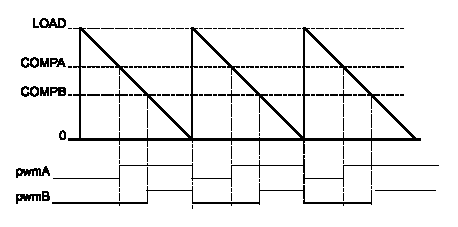
\includegraphics[width=0.8\textwidth] {figuras/Down.eps}
	\caption{PWM modo Down \cite{DATASHEET_TIVA}}
	\label{fig:Down}
\end{figure}

\begin{figure}[H]
	\centering
	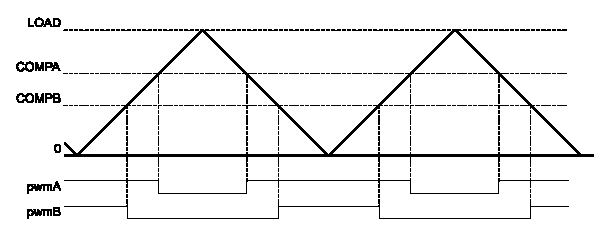
\includegraphics[width=0.8\textwidth] {figuras/UpDown.eps}
	\caption{PWM modo Down \cite{DATASHEET_TIVA}}
	\label{fig:UpDown}
\end{figure}

Tanto na Figura \ref{fig:Down} quanto na Figura \ref{fig:UpDown} os valores de \emph{LOAD}, \emph{COMPA}, \emph{COMPB}, \emph{pwmA} e \emph{pwmB} são referentes aos registradores presente do Tiva - TM4C1294NCPD, responsáveis pela modulação PWM. Tais registradores serão melhor abordados na próxima seção.  

\section{PWM do TM4C1294NCPDT}

O Tiva - TM4C1294NCPD possui um módulo PWM com quatro blocos geradores e seus respectivos blocos de controle, disponibilizando oito saídas PWM.  Através dos blocos de controle é possível escolher qual a polaridade de cada sinal PWM, e o seu respectivo pino. Cada bloco gerador produz 2 sinais PWM com a mesma frequência, porém ambos podem ter \emph{Duty Cicle} independentes ou \emph{Duty Cicle} complementares, com uma intervalo de \emph{Dead Band}. 

Como a maioria das aplicações com PWM é destinada ao chaveamento, o Tiva - TM4C1294NCPD possui não só uma configuração de geração PWM complementar com \emph{Dead Band}, recurso essencial para acionamento de pontes H, como também possui 4 pinos de entrada para um sistema de controle de falha, um para cada gerador PWM.

Para gerar a onda portadora o Tiva possui um contador de 16 bits capaz de realizar contagens no modo \emph{Down} e \emph{UpDown}, sendo possível atualizar o valor da contagem máxima (\emph{LOAD}). Cada um dos geradores PWM possuem ainda dois comparadores distintos (\emph{COMPA} e \emph{COMPB}), responsáveis por gerar os sinais PWM e que podem ser usados para gerar interrupções. 

Quando um comparador está configurado para provocar interrupções esta ocorre toda vez que o valor do comparador selecionado for maior do que o valor de \emph{LOAD}.  A Figura \ref{fig:PWMCountDownMode} demonstra o modo como as os sinais de interrupção são provocados pelos comparadores no modo \emph{Down}, e a Figura \ref{fig:PWMCountUpDownMode} demonstra o mesmo no modo \emph{UpDown}.

\begin{figure}[H]
	\centering
	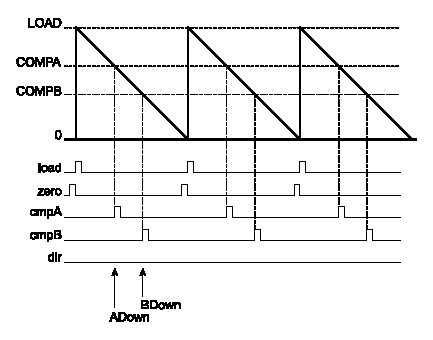
\includegraphics[width=0.8\textwidth] {figuras/PWMCountDownMode.eps}
	\caption{PWM modo Down \cite{DATASHEET_TIVA}}
	\label{fig:PWMCountDownMode}
\end{figure}

\begin{figure}[H]
	\centering
	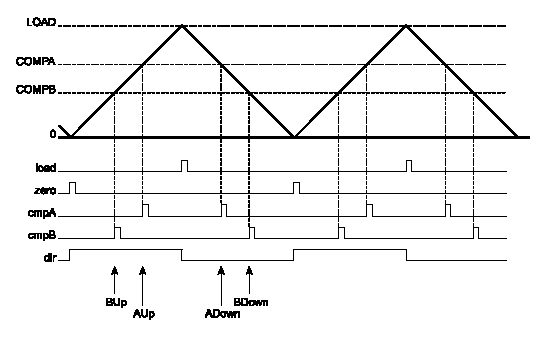
\includegraphics[width=0.8\textwidth] {figuras/PWMCountUpDownMode.eps}
	\caption{PWM modo Down \cite{DATASHEET_TIVA}}
	\label{fig:PWMCountUpDownMode}
\end{figure}

A tabela \ref{tab:CanaisPWM} apresenta os 8 pinos do módulo PWM, sendo estes pinos de saída dos sinais de PWM.  

\begin{center}
	\begin{longtable}{|c|c|c|c|c|}
		\rowcolor[HTML]{000000}
		{\color[HTML]{FFFFFF} Pino} & {\color[HTML]{FFFFFF} $n^{o}$} & {\color[HTML]{FFFFFF} Mux/Função} & {\color[HTML]{FFFFFF} Tipo} & {\color[HTML]{FFFFFF} Descrição}            \\
		M0PWM0    & 42  & PF0 (6) & O & Saída PWM 0\\
		M0PWM1    & 43  & PF1 (6) & O & Saída PWM 1\\
		M0PWM2    & 44  & PF2 (6) & O & Saída PWM 2\\
		M0PWM3    & 45  & PF3 (6) & O & Saída PWM 3\\
		M0PWM4    & 49  & PG0 (6) & O & Saída PWM 4\\
		M0PWM5    & 50  & PG1 (6) & O & Saída PWM 5\\
		M0PWM6    & 63  & PK4 (6) & O & Saída PWM 6\\
		M0PWM7    & 62  & PK5 (6) & O & Saída PWM 7\\
		\hline
		\caption{Canais PWM - Tiva TM4C1294NCPDT \cite{DATASHEET_TIVA} }
		\label{tab:CanaisPWM}
	\end{longtable}
\end{center}

\section{Na TivaWare}

As principais funções de configuração e utilização dos geradores de PWM e suas interrupções são listadas a seguir.

\begin{lstlisting}[style=funcao]
	void PWMClockSet(uint32_t ui32Base,
					 uint32_t ui32Config)
\end{lstlisting}

Configura a frequência do oscilador que alimenta a base de PWM especificada.

\begin{description}
	\item [\ttbu{ui32Base}]\hfill \\
	Base do gerador a ser configurado. Normalmente \textbf{PWM\emph{k}\_BASE}, onde \textbf{\emph{k}} é a letra identificadora do gerador.
	
	\item [\ttbu{ui32Config}]\hfill \\
	Divisão do clock do sistema, para a alimentação do gerador do PWM. É definida no formato \textbf{PWM\_SYSCLK\_DIV\_\emph{k}}, onde \textbf{\emph{k}} pode ser um dos valores: 1, 2, 4, 8, 16, 32 ou 64.
\end{description}

\begin{lstlisting}[style=funcao]
	void PWMGenConfigure(uint32_t ui32Base,
						 uint32_t ui32Gen,
						 uint32_t ui32Config)
\end{lstlisting}

Configura o gerador de PWM especificado.

\begin{description}
	\item [\ttbu{ui32Base}]\hfill \\
	Base do gerador a ser configurado. Normalmente \textbf{PWM\emph{k}\_BASE}, onde \textbf{\emph{k}} é o valor identificador do gerador.
	
	\item [\ttbu{ui32Gen}]\hfill \\
	Gerador a ser configurado. Definido por \textbf{PWM\_GEN\_\emph{k}}, onde \textbf{\emph{k}} pode ser um dos valores: 0, 1, 2 ou 3.
	
	\item [\ttbu{ui32Config}]\hfill \\
	Pacote de parâmetros em formato de OU lógico, onde cada parâmetro é representado no formato \textbf{PWM\_GEN\_MODE\_\emph{k}} e, k pode assumir os valores:
	\begin{itemize}
		\item \textbf{DOWN} ou \textbf{UP\_DOWN} para especificar o modo do contador.
		\item \textbf{SYNC} ou \textbf{NO\_SYNC} para especificar o modo de carregamento do contador e do comparador.
		\item \textbf{DBG\_RUN} ou \textbf{DBG\_STOP} para especificar o comportamento em tempo de depuração.
		\item \textbf{GEN\_NO\_SYNC}, \textbf{GEN\_SYNC\_LOCAL} ou \textbf{GEN\_SYNC\_GLOBAL} para especificar o modo de sincronização do contador do gerador.
		\item \textbf{DB\_NO\_SYNC}, \textbf{DB\_SYNC\_LOCAL} ou \textbf{DB\_SYNC\_GLOBAL} para especificar o modo de sincronização do parâmetro de \emph{deadband}.
		\item \textbf{FAULT\_LATCHED} ou \textbf{FAULT\_UNLATCHED} para especificar se falhas serão travadas ou não.
		\item \textbf{MINPER} ou \textbf{NO\_MINPER} para especificar se há ou não um período mínimo de falha.
		\item \textbf{FAULT\_EXT} ou \textbf{FAULT\_LEGACY} para especificar ou não o uso do suporte de seleção de fonte de falha estendida.
	\end{itemize}
	
\end{description}

\begin{lstlisting}[style=funcao]
	void PWMGenEnable(uint32_t ui32Base,
					   uint32_t ui32Gen)
\end{lstlisting}

Habilita o contador/gerador da base de PWM especificado.

\begin{description}
	\item [\ttbu{ui32Base}]\hfill \\
	Base do gerador a ser habilitado. Normalmente \textbf{PWM\emph{k}\_BASE}, onde \textbf{\emph{k}} é a letra identificadora do gerador.
	
	\item [\ttbu{ui32Gen}]\hfill \\
	Gerador a ser habilitado. Definido por \textbf{PWM\_GEN\_\emph{k}}, onde \textbf{\emph{k}} pode ser um dos valores: 0, 1, 2 ou 3.
\end{description}

\begin{lstlisting}[style=funcao]
	void PWMGenDisable(uint32_t ui32Base,
					   uint32_t ui32Gen)
\end{lstlisting}

Desabilita o contador/gerador da base de PWM especificado.

\begin{description}
	\item [\ttbu{ui32Base}]\hfill \\
	Base do gerador a ser desabilitado. Normalmente \textbf{PWM\emph{k}\_BASE}, onde \textbf{\emph{k}} é a letra identificadora do gerador.
	
	\item [\ttbu{ui32Gen}]\hfill \\
	Gerador a ser desabilitado. Definido por \textbf{PWM\_GEN\_\emph{k}}, onde \textbf{\emph{k}} pode ser um dos valores: 0, 1, 2 ou 3.
\end{description}

\begin{lstlisting}[style=funcao]
	void PWMGenIntTrigEnable(uint32_t ui32Base,
							 uint32_t ui32Gen,
							 uint32_t ui32IntTrig)
\end{lstlisting}

Configura os eventos que causam as interrupções no gerador da base de PWM especificada.

\begin{description}
	\item [\ttbu{ui32Base}]\hfill \\
	Base do gerador a ser configurado. Normalmente \textbf{PWM\emph{k}\_BASE}, onde \textbf{\emph{k}} é a letra identificadora do gerador.
	
	\item [\ttbu{ui32Gen}]\hfill \\
	Gerador a ser configurado. Definido por \textbf{PWM\_GEN\_\emph{k}}, onde \textbf{\emph{k}} pode ser um dos valores: 0, 1, 2 ou 3.
	
	\item [\ttbu{ui32Ints}]\hfill \\
	Pacote de parâmetros em formato de OU binário que especificam as interrupções do PWM. Cada parâmetro é representado no formato \textbf{PWM\_INT\_CNT\_\emph{k}}, onde \textbf{\emph{k}} pode assumir os valores:
	\begin{itemize}
		\item \textbf{ZERO} interrupção acionada ao zerar o contador.
		\item \textbf{LOAD} interrupção acionada ao chegar ao valor máximo do contador
		\item \textbf{AU} interrupção acionada quando o contador é incrementado e alcança o valor especificado no comparador A.
		\item \textbf{AD} interrupção acionada quando o contador é decrementado e alcança o valor especificado no comparador A.
		\item \textbf{BU} interrupção acionada quando o contador é incrementado e alcança o valor especificado no comparador B.
		\item \textbf{BD} interrupção acionada quando o contador é decrementado e alcança o valor especificado no comparador B.
	\end{itemize}
	
\end{description}

\begin{lstlisting}[style=funcao]
	void PWMGenIntClear(uint32_t ui32Base,
						uint32_t ui32Gen,
						uint32_t ui32Ints)
\end{lstlisting}

Limpa as \emph{flags} que marcam a ocorrência das interrupções especificadas no gerador da base de PWM especificado.

\begin{description}
	\item [\ttbu{ui32Base}]\hfill \\
	Base do gerador a ser configurado. Normalmente \textbf{PWM\emph{k}\_BASE}, onde \textbf{\emph{k}} é a letra identificadora do gerador.
	
	\item [\ttbu{ui32Gen}]\hfill \\
	Gerador a ser configurado. Definido por \textbf{PWM\_GEN\_\emph{k}}, onde \textbf{\emph{k}} pode ser um dos valores: 0, 1, 2 ou 3.
	
	\item [\ttbu{ui32Ints}]\hfill \\
	Pacote de parâmetros em formato de OU binário que especificam as interrupções do PWM. Cada parâmetro é representado no formato \textbf{PWM\_INT\_CNT\_\emph{k}}, onde \textbf{\emph{k}} pode assumir os valores:
	\begin{itemize}
		\item \textbf{ZERO} interrupção acionada ao zerar o contador.
		\item \textbf{LOAD} interrupção acionada ao chegar ao valor máximo do contador
		\item \textbf{AU} interrupção acionada quando o contador é incrementado e alcança o valor especificado no comparador A.
		\item \textbf{AD} interrupção acionada quando o contador é decrementado e alcança o valor especificado no comparador A.
		\item \textbf{BU} interrupção acionada quando o contador é incrementado e alcança o valor especificado no comparador B.
		\item \textbf{BD} interrupção acionada quando o contador é decrementado e alcança o valor especificado no comparador B.
	\end{itemize}
	
\end{description}

\begin{lstlisting}[style=funcao]
	void PWMGenIntRegister(uint32_t ui32Base,
						   uint32_t ui32Gen,
						   void (*pfnIntHandler)(void))
\end{lstlisting}

Configura a rotina de tratamento de interrupção do gerador da base de PWM especificada.

\begin{description}
	\item [\ttbu{ui32Base}]\hfill \\
	Base do gerador a ser configurado. Normalmente \textbf{PWM\emph{k}\_BASE}, onde \textbf{\emph{k}} é a letra identificadora do gerador.
	
	\item [\ttbu{ui32Gen}]\hfill \\
	Gerador a ser configurado. Definido por \textbf{PWM\_GEN\_\emph{k}}, onde \textbf{\emph{k}} pode ser um dos valores: 0, 1, 2 ou 3.
	
	\item [\ttbu{pfnIntHandler}]\hfill \\
	Ponteiro da função de tratamento. Esta não deve receber nada como parâmetro e nem retornar nada.
\end{description}

\begin{lstlisting}[style=funcao]
	void PWMGenPeriodSet(uint32_t ui32Base,
						 uint32_t ui32Gen,
						 uint32_t ui32Period)
\end{lstlisting}

Configura o período do sinal no gerador da base de PWM especificada.

\begin{description}
	\item [\ttbu{ui32Base}]\hfill \\
	Base do gerador a ser configurado. Normalmente \textbf{PWM\emph{k}\_BASE}, onde \textbf{\emph{k}} é a letra identificadora do gerador.
	
	\item [\ttbu{ui32Gen}]\hfill \\
	Gerador a ser configurado. Definido por \textbf{PWM\_GEN\_\emph{k}}, onde \textbf{\emph{k}} pode ser um dos valores: 0, 1, 2 ou 3.
	
	\item [\ttbu{ui32Period}]\hfill \\
	Período em formato de valor do contador entre 0 e 2$^n$- 1, onde \emph{n} é o número de bits do contador. Dado pela razão entre a frequência do clock do gerador e a frequência desejada para o PWM.
\end{description}

\begin{lstlisting}[style=funcao]
	void PWMIntEnable(uint32_t ui32Base,
					  uint32_t ui32GenFault)
\end{lstlisting}

Habilita as interrupções para o gerador da base de PWM especificada.

\begin{description}
	\item [\ttbu{ui32Base}]\hfill \\
	Base do gerador a ser configurado. Normalmente \textbf{PWM\emph{k}\_BASE}, onde \textbf{\emph{k}} é a letra identificadora do gerador.
	
	\item [\ttbu{ui32GenFaults}]\hfill \\
	Pacote de parâmetros em formato de OU binário que especificam os geradores que causam interrupções do PWM. Cada parâmetro é representado no formato \textbf{PWM\_INT\_GEN\_\emph{k}}, onde \textbf{\emph{k}} pode assumir os valores: 0, 1, 2, 3.
\end{description}

\begin{lstlisting}[style=funcao]
	void PWMIntDisable(uint32_t ui32Base,
					  uint32_t ui32GenFault)
\end{lstlisting}

Desabilita as interrupções para o gerador da base de PWM especificada.

\begin{description}
	\item [\ttbu{ui32Base}]\hfill \\
	Base do gerador a ser configurado. Normalmente \textbf{PWM\emph{k}\_BASE}, onde \textbf{\emph{k}} é a letra identificadora do gerador.
	
	\item [\ttbu{ui32GenFaults}]\hfill \\
	Pacote de parâmetros em formato de OU binário que especificam os geradores que causam interrupções do PWM. Cada parâmetro é representado no formato \textbf{PWM\_INT\_GEN\_\emph{k}}, onde \textbf{\emph{k}} pode assumir os valores: 0, 1, 2, 3.
\end{description}

\begin{lstlisting}[style=funcao]
	void PWMPulseWidthSet(uint32_t ui32Base,
						  uint32_t ui32PWMOut,
						  uint32_t ui32Width)
\end{lstlisting}

Desabilita as interrupções para o gerador da base de PWM especificada.

\begin{description}
	\item [\ttbu{ui32Base}]\hfill \\
	Base do gerador a ser configurado. Normalmente \textbf{PWM\emph{k}\_BASE}, onde \textbf{\emph{k}} é a letra identificadora do gerador.
	
	\item [\ttbu{ui32PWMOut}]\hfill \\
	Valor que representa a saída de PWM a ser configurada. Representado no formato \textbf{PWM\_OUT\_\emph{k}}, onde \textbf{\emph{k}} pode assumir valores de 0 à 7.
	
	\item [\ttbu{ui32Width}]\hfill \\
	Valor do contador em que o sinal ficará em nível alto.
\end{description}

\section{Exemplo}

Um exemplo de configuração de PWM, utilizando a saída 0 do gerador 0 é apresentada a seguir. É gerada uma onda quadrada de 10 KHz. Outro exemplo, utilizando a interrupção do PWM, pode ser
 encontrado na Seção \ref{sec:exPwm}.
 
\begin{lstlisting}[style=citacao]
	// Configura clock do sistema de 120 MHz
	SysCtlClockFreqSet((SYSCTL_XTAL_25MHZ | SYSCTL_OSC_MAIN | 
		SYSCTL_USE_PLL | SYSCTL_CFG_VCO_480), 120000000);
	// Habilita o PWM 0
	SysCtlPeripheralEnable(SYSCTL_PERIPH_PWM0);
	// Habilita a porta F utilizada no pino de saida de PWM
	SysCtlPeripheralEnable(SYSCTL_PERIPH_GPIOF);

	// Habilita pino de saida1 do PWM 0
	GPIOPinConfigure(GPIO_PF1_M0PWM1);
	// Configura pino F1 como saida do PWM
	GPIOPinTypePWM(GPIO_PORTF_BASE, GPIO_PIN_1);

	// PWM no gerador 0 em modo regressivo, nao sincronizado
	PWMGenConfigure(
		PWM0_BASE, PWM_GEN_0, PWM_GEN_MODE_DOWN |
		PWM_GEN_MODE_NO_SYNC);
	// CLock do gerador e o do sistema dividido por 4
	PWMClockSet(PWM0_BASE, PWM_SYSCLK_DIV_4);
	// Periodo de 10 KHz -> 120000000 / 4 / 10000
	PWMGenPeriodSet(PWM0_BASE, PWM_GEN_0, 3000);
	// Largura de pulso de 50% -> 3000 * 0.5
	PWMPulseWidthSet(PWM0_BASE, PWM_OUT_1, 1500);
	// Habilita gerador 0
	PWMGenEnable(PWM0_BASE, PWM_GEN_0);
	// Saidas de PWM a serem modificadas
	PWMOutputState(PWM0_BASE,
		(PWM_OUT_0_BIT | PWM_OUT_1_BIT), true);
	
	// Habilita interrupcao do gerador 0
	PWMIntEnable(PWM0_BASE, PWM_INT_GEN_0);
	// Habilita interrupcao do PWM 0
	IntEnable(INT_PWM0_0);
	// Interrupcao disparada no estouro do contador
	PWMGenIntTrigEnable(PWM0_BASE, PWM_GEN_0, 
		PWM_INT_CNT_LOAD);
\end{lstlisting}

\chapter{Temporizador de Propósito Geral}

Contadores 
\section{Modos de Funcionamento}

\section{Temporizador no TM4C1294NCPDT}

\section{Exemplo}

% \setcounter{minitocdepth}{1}

\chapter{Exemplos de aplicação}
Esta seção apresenta alguns exemplos práticos de implementação no TivaWare. É importante ressaltar que esses exemplos foram desenvolvidos para o TM4C1294NCPDT. Sendo assim, podem haver incompatibilidades presentes no carregamento destes códigos para algum outro hardware diferente, mesmo suportado pelo TivaWare.

\section{Listagem de Periféricos pela UART}

O seguinte software, implementa uma comunicação UART na base de UART 0 do microcontrolador. Ao receber bytes, e detectado algum caractere 'p', é imprimido uma lista com os periféricos disponíveis no microcontrolador. Se for algum outro caractere, somente é exibida uma mensagem informativa.

\lstset{language=C,caption={Código de exemplo},label=DescriptiveLabel}
\lstinputlisting{codigo/UARTecho.c}


\bibliographystyle{abbrv}
\bibliography{bibliografia.bib}

\end{document}